%%%%%%%%%%%%%%%%%%%%%%%%%%%%%%%%%%%%%%%%%%%%%%%%%%%%%%%%%%%%%%%%%%%%%%%%%%%%%%%%
%% Plantilla de memoria en LaTeX para la ETSIT - Universidad Rey Juan Carlos
%%
%% Por Gregorio Robles <grex arroba gsyc.urjc.es>
%%     Grupo de Sistemas y Comunicaciones
%%     Escuela Técnica Superior de Ingenieros de Telecomunicación
%%     Universidad Rey Juan Carlos
%% (muchas ideas tomadas de Internet, colegas del GSyC, antiguos alumnos...
%%  etc. Muchas gracias a todos)
%%
%% La última versión de esta plantilla está siempre disponible en:
%%     https://github.com/gregoriorobles/plantilla-memoria
%%
%% Para obtener PDF, ejecuta en la shell:
%%   make
%% (las imágenes deben ir en PNG o JPG)

%%%%%%%%%%%%%%%%%%%%%%%%%%%%%%%%%%%%%%%%%%%%%%%%%%%%%%%%%%%%%%%%%%%%%%%%%%%%%%%%

\documentclass[a4paper, 12pt]{book}
%\usepackage[T1]{fontenc}

\usepackage[a4paper, left=2.5cm, right=2.5cm, top=3cm, bottom=3cm]{geometry}
\usepackage{times}
\usepackage[utf8]{inputenc}
\usepackage[spanish]{babel} % Comenta esta línea si tu memoria es en inglés
\usepackage{url}
%\usepackage[dvipdfm]{graphicx}
\usepackage{graphicx}
\usepackage{float}  %% H para posicionar figuras
\usepackage[nottoc, notlot, notlof, notindex]{tocbibind} %% Opciones de índice
\usepackage{latexsym}  %% Logo LaTeX

\title{Memoria del Proyecto}
\author{Iván Miguel Molinero}

\renewcommand{\baselinestretch}{1.5}  %% Interlineado

\begin{document}

\renewcommand{\refname}{Bibliografía}  %% Renombrando
\renewcommand{\appendixname}{Apéndice}

%%%%%%%%%%%%%%%%%%%%%%%%%%%%%%%%%%%%%%%%%%%%%%%%%%%%%%%%%%%%%%%%%%%%%%%%%%%%%%%%
% PORTADA

\begin{titlepage}
\begin{center}
\includegraphics[scale=0.8]{img/URJ_logo_Color_POS.png}

\vspace{1.75cm}

\Large
GRADO EN INGENIERÍA EN SISTEMAS AUDIOVISUALES
Y MULTIMEDIA

\vspace{0.4cm}

\large
Curso Académico 2022/2023

\vspace{0.8cm}

Trabajo Fin de Grado

\vspace{2.5cm}

\LARGE
EVALUACIÓN SISTEMÁTICA DE PROYECTOS DE SOFTWARE LIBRE

\vspace{4cm}

\large
Autor : Iván Miguel Molinero \\
Tutor : Dr. Gregorio Robles Martínez
\end{center}
\end{titlepage}

\newpage
\mbox{}
\thispagestyle{empty} % para que no se numere esta pagina


%%%%%%%%%%%%%%%%%%%%%%%%%%%%%%%%%%%%%%%%%%%%%%%%%%%%%%%%%%%%%%%%%%%%%%%%%%%%%%%%
%%%% Para firmar
\clearpage
\pagenumbering{gobble}
\chapter*{}

\vspace{-4cm}
\begin{center}
\LARGE
\textbf{Trabajo Fin de Grado/Máster}

\vspace{1cm}
\large
Evaluación Sistemática de Proyectos de Software Libre

\vspace{1cm}
\large
\textbf{Autor :} Iván Miguel Molinero \\
\textbf{Tutor :} Dr. Gregorio Robles Martínez

\end{center}

\vspace{1cm}
La defensa del presente Proyecto Fin de Carrera se realizó el día \qquad$\;\,$ de \qquad\qquad\qquad\qquad \newline de 202X, siendo calificada por el siguiente tribunal:


\vspace{0.5cm}
\textbf{Presidente:}

\vspace{1.2cm}
\textbf{Secretario:}

\vspace{1.2cm}
\textbf{Vocal:}


\vspace{1.2cm}
y habiendo obtenido la siguiente calificación:

\vspace{1cm}
\textbf{Calificación:}


\vspace{1cm}
\begin{flushright}
Fuenlabrada, a \qquad$\;\,$ de \qquad\qquad\qquad\qquad de 202X
\end{flushright}

%%%%%%%%%%%%%%%%%%%%%%%%%%%%%%%%%%%%%%%%%%%%%%%%%%%%%%%%%%%%%%%%%%%%%%%%%%%%%%%%
%%%% Dedicatoria

\chapter*{}
\pagenumbering{Roman} % para comenzar la numeracion de paginas en numeros romanos
\begin{flushright}
\textit{Hazlo o no lo hagas, \\
pero no lo intentes. \\
Maestro Yoda}
\end{flushright}

%%%%%%%%%%%%%%%%%%%%%%%%%%%%%%%%%%%%%%%%%%%%%%%%%%%%%%%%%%%%%%%%%%%%%%%%%%%%%%%%
%%%% Agradecimientos

\chapter*{Agradecimientos}
%\addcontentsline{toc}{chapter}{Agradecimientos} % si queremos que aparezca en el índice
\markboth{AGRADECIMIENTOS}{AGRADECIMIENTOS} % encabezado 

Siete años después he conseguido llegar hasta aquí, aunque hubo momentos en los que quise abandonar, nunca me rendí y he logrado terminar la carrera. Esto no hubiera sido posible, en primer y principal lugar, sin mis padres. Siempre han estado ahí, apoyándome, animándome, pagándome todo lo que necesitara, valiera lo que valiera como el ordenador desde el que escribo estas líneas o las asignaturas en las que llegué a tercera matrícula o incluso quinta. Gracias, Jose y Yoli, gracias, papá y mamá, sin vosotros esto hubiera sido imposible. Os quiero.
De esta carrera también me llevo a una nueva familia. ¿Quién iba a decirme que terminaría amando lo que en 2017 describía como una pedanía? Hablo de Jaén y del hermano y hermana que me llevo para siempre. Gracias por confiar en mí incluso cuando ni yo lo hacía. Siempre habéis estado ahí para mí, escuchando cada audio durase lo que durase, hablase de lo que hablase, desde lo enfadado que estaba por que había perdido el Madrid hasta mis penas y alegrías. Me enseñasteis lo que es una amistad de verdad, gracias. Agradecer también a personas que pasaron por mi vida durante esta etapa y que me enseñaron a ''no ocuparme antes de ocuparme'', a mi psicóloga que me enseñó que casi nada esta vida es catastrófico y me dio las herramientas para poder sacar mi mejor versión cuando ni yo sabía lo que me pasaba. También quiero agradecer a todos los compañeros que he tenido en la carrera, entre todos nos hicimos la vida un poco más fácil. Gracias, claro, a mi equipo, el Real Madrid que me enseñó a luchar ''hasta el final'' como reza el tatuaje que llevo en el brazo.
Para terminar, dar las gracias al C.E.I.P. Pío Baroja, al I.E.S. Manuel de Falla de Móstoles y a la Universidad Rey Juan Carlos de Fuenlabrada por formarme como persona y como profesional así como a los espectaculares profesores que he tenido a lo largo de mi vida como Sara, Diego, Susana, Juan y, en especial, mi tutor del TFG quien desde el minuto uno me transmitió su pasión por Python y la programación. Gracias a todos y a por más.

%%%%%%%%%%%%%%%%%%%%%%%%%%%%%%%%%%%%%%%%%%%%%%%%%%%%%%%%%%%%%%%%%%%%%%%%%%%%%%%%
%%%% Resumen

\chapter*{Resumen}
%\addcontentsline{toc}{chapter}{Resumen} % si queremos que aparezca en el índice
\markboth{RESUMEN}{RESUMEN} % encabezado

Inicié este proyecto con el objetivo de seguir creciendo como desarrollador y, a la vez, crear una herramienta que fuera de utilidad para más desarrolladores como yo. A la hora de buscar herramientas en Github impresiona la gran cantidad de ellas que hay y, para desarolladores novatos como yo (y no tan novatos) es difícil distinguir las mejores opciones.

Es por eso que nació este proyecto, para permitir a los desarrolladores analizar los respositorios de una manera más rápida y eficaz. El objetivo final sería poder analizar una gran cantidad de repositorios al mismo tiempo con esta aplicación.

Estos objetivos no son nuevos, ya los han tenido diferentes proyectos como OpenBRR el cual se eligió usar y ampliar ya que se centra en los aspectos más importantes de los proyectos. Además, es de código abierto, lo que siempre facilita las cosas.

Pero el uso de esta aplicación no está centrado solo en desarrolladores noveles, también se puede usar en el ámbito educativo para que los profesores puedan elegir qué repositorios recomendar a sus alumnos. 

Finalmente, indicar que este proyecto se ha realizado con Python, Django, HTML, CSS  y JS, tecnologías que he ido aprendiendo durante mi estancia en la universidad.

%%%%%%%%%%%%%%%%%%%%%%%%%%%%%%%%%%%%%%%%%%%%%%%%%%%%%%%%%%%%%%%%%%%%%%%%%%%%%%%%
%%%% Resumen en inglés

\chapter*{Summary}
%\addcontentsline{toc}{chapter}{Summary} % si queremos que aparezca en el índice
\markboth{SUMMARY}{SUMMARY} % encabezado

I started this project with the aim of continuing to grow as a developer and, at the same time, to create a tool that would be useful for more developers like me. When looking for tools on Github, it is impressive how many tools there are and, for novice developers like me (and not so novice) it is difficult to distinguish the best options.

That's why this project was born, to allow developers to analyse repositories in a faster and more efficient way. The ultimate goal would be to be able to analyse a large number of repositories at the same time with this application.

These goals are not new, they have already been achieved by different projects such as OpenBRR which was chosen to use and extend as it focuses on the most important aspects of the projects. Moreover, it is open source, which always makes things easier.

But the use of this application is not only focused on novice developers, it can also be used in the educational field so that teachers can choose which repositories to recommend to their students. 

Finally, this project has been done with Python, Django, HTML, CSS and JS, technologies that I have been learning during my stay at the university.

%%%%%%%%%%%%%%%%%%%%%%%%%%%%%%%%%%%%%%%%%%%%%%%%%%%%%%%%%%%%%%%%%%%%%%%%%%%%%%%%
%%%%%%%%%%%%%%%%%%%%%%%%%%%%%%%%%%%%%%%%%%%%%%%%%%%%%%%%%%%%%%%%%%%%%%%%%%%%%%%%
% ÍNDICES %
%%%%%%%%%%%%%%%%%%%%%%%%%%%%%%%%%%%%%%%%%%%%%%%%%%%%%%%%%%%%%%%%%%%%%%%%%%%%%%%%

% Las buenas noticias es que los índices se generan automáticamente.
% Lo único que tienes que hacer es elegir cuáles quieren que se generen,
% y comentar/descomentar esa instrucción de LaTeX.

%%%% Índice de contenidos
\tableofcontents 
%%%% Índice de figuras
\cleardoublepage
%\addcontentsline{toc}{chapter}{Lista de figuras} % para que aparezca en el indice de contenidos
\listoffigures % indice de figuras
%%%% Índice de tablas
%\cleardoublepage
%\addcontentsline{toc}{chapter}{Lista de tablas} % para que aparezca en el indice de contenidos
%\listoftables % indice de tablas


%%%%%%%%%%%%%%%%%%%%%%%%%%%%%%%%%%%%%%%%%%%%%%%%%%%%%%%%%%%%%%%%%%%%%%%%%%%%%%%%
%%%%%%%%%%%%%%%%%%%%%%%%%%%%%%%%%%%%%%%%%%%%%%%%%%%%%%%%%%%%%%%%%%%%%%%%%%%%%%%%
% INTRODUCCIÓN %
%%%%%%%%%%%%%%%%%%%%%%%%%%%%%%%%%%%%%%%%%%%%%%%%%%%%%%%%%%%%%%%%%%%%%%%%%%%%%%%%

\cleardoublepage
\chapter{Introducción}
\label{chap:introducción}
\label{sec:intro} % etiqueta para poder referenciar luego en el texto con ~\ref{sec:intro}
\pagenumbering{arabic} % para empezar la numeración de página con números

Actualmente se comparten muchos proyectos de software libre en Internet en general y en Github~\cite{website:GitHub}\footnote{\url{https://github.com/}} en particular. Algunos ejemplos de proyectos que se comparten son paquetes de Python que
ayudan a desarrolladores a no tener que "reinventar la rueda", es decir, que si necesitas hacer un proyecto que lea URLs en uno de sus pasos (por ejemplo) y alguien ya ha hecho un paquete para
ello, debes usar ese paquete para poder avanzar en tu proyecto de una forma más rápida y eficaz.

Un proyecto de software libre es un desarrollo que es público; los demás desarrolladores pueden verlo y mejorarlo a través de Pull Request y también descargarlo gratuitamente para su uso por eso muchos usuarios lo prefieren a proyectos de código cerrado.

Ahora bien, en Github se comparten infinidad de proyectos de software libre y no siempre es fácil distinguir entre los que son buenos y los que no lo son tanto: ¿cuál es más seguro? o ¿cuál es más eficiente?
Para resolver estas y más preguntas es que, gracias al paquete PyGithub\footnote{\url{https://github.com/pygithub/pygithub}}, he desarrollado esta aplicación web que permite al usuario introducir el nombre de un repositorio y analizarlo según los parámetros que más
le convengan.

El proyecto\cite{website:RepositorioTFG}  nace como una extensión de OpenBRR\footnote{\url{https://link.springer.com/chapter/10.1007/978-3-642-13244-5_18}} que es una forma de analizar proyectos en función a los siguientes 7 parámetros: funcionalidad, calidad, soporte, comunidad, adopción y usabilidad.
A estos parámetros se les asigna un peso y a partir de ahí, da una calificación final sobre 5 del proyecto. A parte de OpenBRR existen otras formas de analizar proyectos como OSMM, OpenBQR o MOSST entre muchos otros pero me decanté por esta opción al ser la que más se 
centraba en analizar los proyectos de software libre.

Esta herramienta ayudará a docentes y desarrolladores a distinguir entre los miles de repositorios de Github cuáles son los que merecen la pena agilizando mucho la búsqueda. Pongamos un ejemplo práctico para que se entienda mejor: un desarrollador busca un paquete
que realice una función específica para su proyecto pero si tiene que buscar entre las miles de opciones cuál es la mejor, tardaría un tiempo excesivo ya que tendría que analizar cada código por si mismo (con todo lo que ello supone como entenderlo si no está bien comentado),
buscar vulnerabilidades, descargarlo, probarlo , etc. En cambio, gracias a este proyecto podrá buscar su mejor opción configurando el análisis según le convenga pudiendo poner el foco solo en seguridad, en seguridad y funcionalidad o en los 7 apartados que tiene OpenBRR.


\section{Estructura de la memoria}
\label{sec:estructura}

\begin{itemize}
  \item \textbf{Capítulo~\ref{chap:introducción}:} se explica brevemente el origen del proyecto, sus bases y funcionamiento .
  
  \item \textbf{Capítulo~\ref{chap:objetivos}:} se muestran los objetivos del proyecto.
  
  \item \textbf{Capítulo~\ref{chap:estado}:} se explica cada tecnología usada en este proyecto.
  
  \item \textbf{Capítulo~\ref{chap:diseño}:} aquí se entra en detalle en el funcionamiento de la aplicación.
  
  \item \textbf{Capítulo~\ref{chap:experimentos}:} se muestran los diferentes experimentos y se prueba el correcto funcionamiento de la aplicación.
  
  \item \textbf{Capítulo~\ref{chap:resultados}:} se explican los resultados obtenidos poniendo de prueba varios repositorios.
  
  \item \textbf{Capítulo~\ref{chap:conclusiones}:} se indican los resultados conseguidos y la solución a los objetivos no conseguidos.
  
\end{itemize}



%%%%%%%%%%%%%%%%%%%%%%%%%%%%%%%%%%%%%%%%%%%%%%%%%%%%%%%%%%%%%%%%%%%%%%%%%%%%%%%%
%%%%%%%%%%%%%%%%%%%%%%%%%%%%%%%%%%%%%%%%%%%%%%%%%%%%%%%%%%%%%%%%%%%%%%%%%%%%%%%%
% OBJETIVOS %
%%%%%%%%%%%%%%%%%%%%%%%%%%%%%%%%%%%%%%%%%%%%%%%%%%%%%%%%%%%%%%%%%%%%%%%%%%%%%%%%

\cleardoublepage % empezamos en página impar
\chapter{Objetivos} % título del capítulo (se muestra)
\label{chap:objetivos} % identificador del capítulo (no se muestra, es para poder referenciarlo)

\section{Objetivo general} % título de sección (se muestra)
\label{sec:objetivo-general} % identificador de sección (no se muestra, es para poder referenciarla)

Mi trabajo de fin de grado consiste en crear una aplicación web que analice repositorios de Github para darles una calificación sobre 5 basándose en los parámetros de OpenBRR.


\section{Objetivos específicos}
\label{sec:objetivos-especificos}

A la hora de realizar este proyecto, he abordado los siguientes objetivos específicos:

\begin{itemize}
	\item Estudiar, aprender y utilizar Django\footnote{\url{https://www.djangoproject.com/}}.

	\item Estudiar qué es OpenBRR y saber cómo analizar un código para poder calificar cada uno de sus parámetros.
	
	\item Analizar el paquete PyGithub en busca de las funciones que necesitaba para analizar repositorios.

	\item Rellenar y enviar formularios con Django.

	\item Manipular los datos enviados por el usuario y enviar los resultados.

	\item Probar el proyecto tanto con repositorios vacíos, como con repositorios teóricamente buenos para comprobar si los resultados eran coherentes.

	\item Solucionar errores como que el usuario introduzca un repositorio que no exista.

	\item Introducir mejoras tales como permitir al usuario introducir una dirección de correo electrónico para que le lleguen los resultados ahí también.

	\item Probar aún más repositorios haciendo que la aplicación se centrase en diferentes parámetros para comprobar que hacía un correcto análisis.
\end{itemize}


\section{Planificación temporal}
\label{sec:planificacion-temporal}

El proyecto se empezó a pensar a finales de Febrero de 2022 pero no fue hasta el verano de ese año que se empezó a trabajar en serio en él ya que anteriormente tenía que compaginarlo con las prácticas externas y no disponía del tiempo necesario. 
De Marzo a Junio de 2022 dedicaba las mañanas de los sábados y domingos a investigar qué era OpenBRR, en qué consistía y cómo podía usarlo para este proyecto. Asimismo mi tutor me recomendó usar el paquete Perceval\footnote{\url{https://perceval.readthedocs.io/en/latest/perceval/git.html}} de Python para analizar los repositorios de GitHub pero tras investigar por mi cuenta di con el paquete PyGithub el cual analizaba los repositorios de una forma más rápida y cómoda para el desarrollador ya que únicamente con introducir el nombre del repositorio es capaz de sacar todos los datos necesarios.

Durante el verano, pasaba las mañanas de lunes a viernes trabajando en el TFG y conseguí entender el funcionamiento completo de PyGithub así como analizar todos los datos que me devolvía y relacionarlos con los 7 parámetros de OpenBRR intentando que cada dato perteneciera al parámetro que más le correspondiera.

En el mes de Septiembre decidí implementar Django en la aplicación para ser capaz de leer, manipular y crear páginas web a través de las peticiones del usuario. No tenía conocimientos sobre esta tecnología así que usé los tutoriales de DjangoGirls\footnote{\url{https://djangogirls.org/es/}}\cite{website:DjangoGirls} para aprender a utilizarla dedicando 3 tardes de lunes a viernes y las mañanas de los sábados y domingos.

Finalmente, de Octubre de 2022 a Enero de 2023, empecé con el desarrollo de la aplicación web dedicando el mismo reparto de tiempo que para aprender Django ya que tenía clases de la universidad por las mañanas salvo en las vacaciones de Navidad que le dediqué todas las mañanas sin excepción. Durante el desarrollo surgieron varias dudas como qué datos asignar a qué parámetros y, sobretodo, qué peso asignarle a cada dato pero tras varias reuniones con mi tutor decidimos que el usuario pudiera manejar los pesos a su antojo para así poder centrarse en analizar los repositorios de la forma que más le convenga.
A finales de Diciembre comencé a hacer pruebas con repositorios profesionales como el propio de PyGithub o los de myTeachingURJC\footnote{\url{https://github.com/myTeachingURJC}} (los cuales son utilizados por los profesores de la universidad para compartir contenido de sus asignaturas) y con repositorios de peor calidad como mis primeros repositorios en busca de evaluaciones coherentes y algún error. Para principios de Enero la aplicación ya era funcional pero no tenía ningún tipo de estilo así que dediqué el resto del tiempo a personalizar su aspecto, así como a corregir y controlar errores que surgían durante las diferentes pruebas que realizaba.
Por tanto, dediqué las mañanas de finales de Enero y todo Febrero para la realización de la memoria con el objetivo de poder presentar el proyecto en Marzo.

%%%%%%%%%%%%%%%%%%%%%%%%%%%%%%%%%%%%%%%%%%%%%%%%%%%%%%%%%%%%%%%%%%%%%%%%%%%%%%%%
%%%%%%%%%%%%%%%%%%%%%%%%%%%%%%%%%%%%%%%%%%%%%%%%%%%%%%%%%%%%%%%%%%%%%%%%%%%%%%%%
% ESTADO DEL ARTE %
%%%%%%%%%%%%%%%%%%%%%%%%%%%%%%%%%%%%%%%%%%%%%%%%%%%%%%%%%%%%%%%%%%%%%%%%%%%%%%%%

\cleardoublepage
\chapter{Estado del arte}
\label{chap:estado}

Para la realización de este proyecto se ha utilizado Python, PyGithub, Github, Django, HTML, CSS, Javascript y OpenBRR.

\section{Python}
\label{sec:python}

Python\cite{website:Python} es un lenguaje de programación interpretado que le da importancia a la legibilidad del código teniendo una sintaxis muy limpia. Está orientado a objetos y permite ser un buen lenguaje para aprender a programar ya que tiene una curva de aprendizaje muy suave qracias a su sintaxis muy cercana al lenguaje humano. En un lenguaje de código abierto, lo que le permite estar en constante mejora por parte de los usuarios y ser adaptado para diferentes usos como el Machine Learning.

Python fue creado por Guido van Rossum en 1991 mientras trabajaba en el sistema operativo Amoeba\footnote{\url{https://www.cs.vu.nl/pub/amoeba/}} teniendo como objetivo controlar excepciones y manejar interfaces de dicho sistema operativo. A finales del año 2000 nació Python 2.0 el cual soportaba Unicode por primera vez y empezó a ser desarrollado por la comunidad bajo la mirada de Guido. Finalmente, en 2008 se lanzó Python 3.0 siendo la versión más completa de Python pero incompatible con las anteriores por lo que muchas características se implementaron también en Python 2.6.

La filosofía de Python se basa en los siguientes puntos para hacer la vida más fácil al desarrollador:

 \begin{itemize}
 	\item Hermoso es mejor que feo.
	\item Explícito es mejor que implícito.
 	\item Simple es mejor que complejo.
 	\item Plano es mejor que anidado.
 	\item Disperso es mejor que denso.
 	\item El código legible cuenta.
	\item Casos especiales no son lo suficientemente 	especiales para romper las reglas.
	\item Casi siempre lo práctico vence a lo formal
	\item Los errores no deben pasar nunca desapercibidos, a menos que se
especifique este comportamiento.
	\item Ante una ambigüedad, descarte la tentación a adivinar.
	\item Debe haber una, y preferentemente una sola, manera obvia de lograr.
algo, aunque esta generalmente no está clara a primera vista a menos
que seas un genio.
	\item Ahora es mejor que nunca, aunque en muchas ocasiones nunca es
mejor que ahora mismo.
	\item Si la implementación es difícil de explicar, entonces es una mala idea.
	\item Si la implementación es fácil de explicar, entonces pudiera ser una
buena idea.
	\item Los espacios de nombre son una buena idea, hagamos más de eso.
 \end{itemize}
 
 Para finalizar, aquí podemos ver un ejemplo de un fragmento de código en Python correspondiente a un desarrollo que hice por mi cuenta\footnote{\url{https://github.com/ivanmiguelmolinero/Python2D}} : 
 
 {\footnotesize
\begin{verbatim}
  class MiCuchillo(Sprite):
    def __init__(self, image, dir, x, y):
        super().__init__(image)
        self.position = (x, y)
        self.direccion = dir
        self.cshape = AARectShape(self.position, self.width/5, self.height/5)

    def update(self, dt):
        coor_cuchillo = manejador_scroll.world_to_screen(self.x, self.y)[0]
        if coor_cuchillo > 1280 or coor_cuchillo < 0:
            self.kill()
        if self.direccion == 'd':
            self.position += Vector2(20, 0)
        if self.direccion == 'i':
            self.position -= Vector2(20, 0)
        self.cshape.center = Vector2(self.position[0], self.position[1])
\end{verbatim}
}

\section{PyGithub}
\label{sec:pygithub}

PyGithub\cite{website:Pygithub} se trata de la librería utilizada en la aplicación para analizar los datos del repositorio. Adicionalmente, también permite administrar recursos de Github como repositorios, perfiles de usuario y organizaciones. Es una librería de código abierto lo que permite que esté en constante mejora y desarrollo por parte de la comunidad. 

Algunas funciones de interés son:

\subsection{get\textunderscore repository()}

Esta función permite obtener todos los datos del repositorio únicamente pasándole el nombre del repositorio. Ejemplo de uso sacado directamente de este proyecto:

 {\footnotesize
\begin{verbatim}
  # Obtenemos el repositorio introducido por el usuario
    repo = get_repository(request.GET['text'])
\end{verbatim}
}

\subsection{get\textunderscore wiki()}

Esta función es un ejemplo de los datos que nos permite analizar PyGithub. En concreto, ``getwiki()´´ nos devuelve si el repositorio en cuestión tiene wiki o no. Otros ejemplos de funciones de este tipo son ``repo.homepage´´, ``repo.subscriberscount´´, ``repo.getcommits().totalCount´´...

\section{Github}
\label{sec:github}

Github es una herramienta esencial para ingenieros de software que consiste en un servicio basado en la nube donde los desarrolladores suben sus proyectos de código abierto a unos repositorios para compartirlos con la comunidad, permitiendo así realizar cambios y mejoras en el proyecto. Se ha convertido en una herramienta muy popular llegando a alojar más de 100 millones de repositorios.

Github fue desarrollado por Chris Wanstrath, P. J. Hyett, Tom Preston-Werner y Scott Chacon usando Ruby on Rails, y comenzó a funcionar en 2008. Desde 2018 pertenece a Microsoft.

A continuación se explican los diferentes mecanismos que permiten que funcione Github.

\subsection{Repositorios}

Lugar donde los desarrolladores suben sus proyectos. Por ejemplo, este proyecto está subido en el repositorio ``ivanmiguelmolinero/TFG´´.

\subsection{Pull request}

Es la funcionalidad que permite a los desarrolladores colaborar entre ellos sugiriendo cambios del programa en cuestión.

\subsection{Commits}

Funcionalidad que permite realizar y subir al repositorio cambios en el proyecto junto con un breve mensaje descriptivo. Se puede ejecutar mediante la interfaz de un editor de código con VSCode\footnote{\url{https://code.visualstudio.com/}} o bien ejecutando ``git commit -m [mensaje descriptivo entre comillas]´´ en una ventana de comandos.

\subsection{Wiki}

Sección del repositorio donde se explica la funcionalidad del proyecto, el manual de usuario y los diferentes cambios que se van implementando. Muchos proyectos también usan el README del repositorio para estas funcionalidades.

\section{Django}
\label{sec:django}

Django es un framework de Python de alto nivel que fue creado para gestionar páginas web facilitando la creación de sitios web complejos. Fue lanzado inicialmente en Julio de 2005. 

La distribución principal de Django permite aplicaciones con un sistema de comentarios, herramientas para juntar contenido vía RSS\footnote{\url{https://www.rssboard.org/rss-specification}} o Atom\footnote{\url{https://www.ietf.org/rfc/rfc4287}} , plantillas que permiten gestionar páginas de contenido sin necesidad de escribir controladores o vistas de esas páginas  y un sistema de redirección de URLs.

Las características principales de Django son:

\begin{itemize}
	\item Framework muy rápido, es decir, permite a los desarrolladores terminar sus proyectos lo más rápido posible.
	\item Es muy seguro: ayuda a evitar los errores de seguridad más comunes.
	\item Es muy escalable: a medida que crece la aplicación da facilidades para añadirle las nuevas funcionalidades.
\end{itemize} 

\section{HTML}
\label{sec:html}

HTML\cite{website:HTML}  (lenguaje de marcas de hipertexto) es el componente más básico de una página web. Es usado para estructurar el contenido de la misma. Normalmente se utiliza junto con CSS y Javascript que se explicarán en los siguientes apartados.
Hipertexto se refiere a los enlaces que conectan las páginas web entre sí.

Un elemento HTML se distingue de otro mediante etiquetas que se definen entre los símbolos $"<"$ y $">"$. 

En la siguiente figura se puede ver un ejemplo de HTML
\begin{figure}
  \centering
  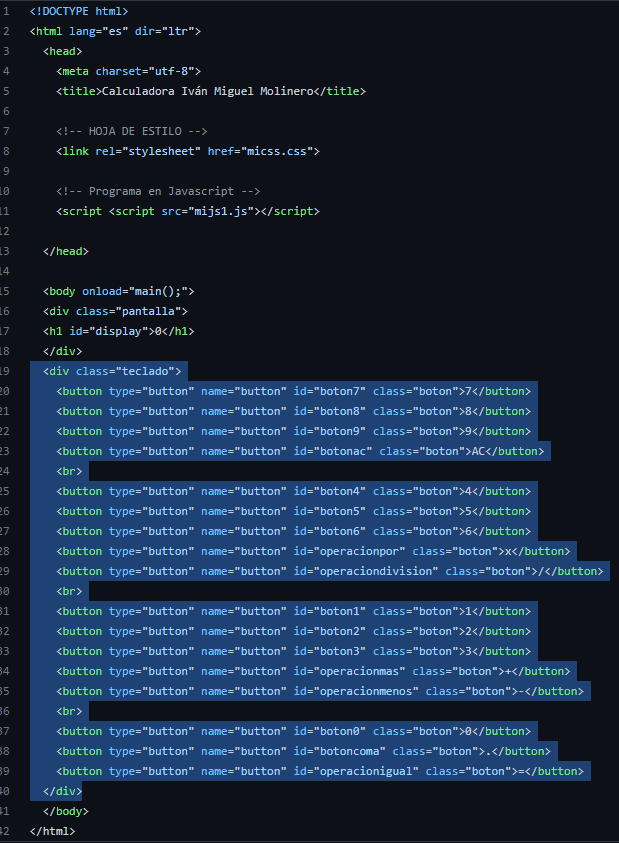
\includegraphics[width=10cm, keepaspectratio]{img/html.png}
  \caption{Fragmento HTML}\label{fig:html}
\end{figure}
\\

\section{CSS}
\label{sec:CSS}

CSS\cite{website:CSS} (del inglés Cascading Style Sheets) es utilizado para dar estilo a las páginas web creadas con HTML o XML. Ha tenido varias versiones pero es desde CSS3 que su alcance es tal que cada módulo empezó a mostrar varias diferencias por lo que el W3C\footnote{\url{https://www.w3.org/}}  decidió empezar a realizar capturas de las últimas especificaciones estables.

Su sintaxis más básica consiste en hacer referencia a las diferentes etiquetas de HTML y definir su estilo entre corchetes. Por ejemplo:

\begin{verbatim}
div {
    text-align: center;
}

img {
  height: 20px;
  margin-left: 0px;
}
\end{verbatim}

\section{Javascript}
\label{sec:Javascript}

Javascript\cite{website:Javascript} (abreviado JS) es un lenguaje de programación ligero, interpretado y compilado ``just-in-time´´. Se usa para secuencias de comandos en páginas web aunque también se utiliza en otros entornos como Node.js\footnote{\url{https://developer.mozilla.org/es/docs/Glossary/Node.js}}.

Se originó en el año 1995 para el navegador Netscape como una forma de agregar programas a páginas web. Desde entonces, el lenguaje ha sido adoptado por todos los demás navegadores gráficos principales. Ha hecho posibles las aplicaciones web modernas, aplicaciones con las que puede interactuar directamente sin hacer una recarga de página para cada acción.

Algunas de las características de Javascript son las siguientes:

\begin{itemize}
	\item Lenguaje del lado del cliente
	\item Orientado a objetos
	\item De tipado débil o no tipado
	\item De alto nivel
	\item Lenguaje interpretado
	\item Muy utilizado por los desarrolladores\\
\end{itemize}

\section{OpenBRR}
\label{sec:openbrr}

OpenBRR\cite{website:OpenBRR} (del inglés Business Readiness Rating) es un modelo de evaluación de software libre. Su objetivo es estandarizar una fórmula de evaluación de software. Este método fue patrocinado por el Centro de Investigación de Código abierto e Intel.

Se considera necesario ya que proporciona a las compañías una forma segura, estandarizada y eficaz de evaluar un software antes de adoptarlo. Hasta el momento ha permitido a compañías tanto elegir un software ideal para misiones críticas como descartar otros que a primera vista parecían buenos pero que después de analizarlos dieron con graves problemas de seguridad.

El esquema de análisis se puede ver en la figura 3.2. Aparte de los parámetros que aparecen en la figura se decidió introducir el parámetro de seguridad al considerarse de importancia también.

\begin{figure}
  \centering
  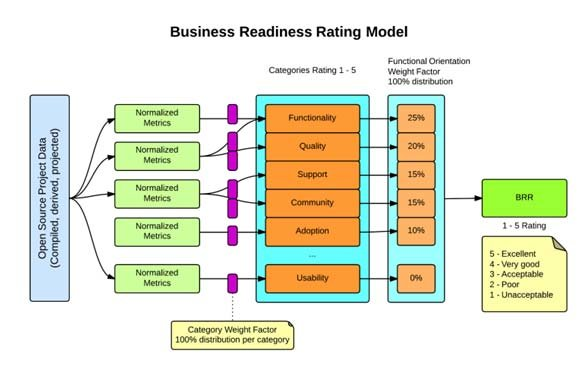
\includegraphics[width=14cm, keepaspectratio]{img/openbrr.png}
  \caption{Esquema de análisis de OpenBRR}\label{fig:OpenBRR}
\end{figure}


%%%%%%%%%%%%%%%%%%%%%%%%%%%%%%%%%%%%%%%%%%%%%%%%%%%%%%%%%%%%%%%%%%%%%%%%%%%%%%%%
%%%%%%%%%%%%%%%%%%%%%%%%%%%%%%%%%%%%%%%%%%%%%%%%%%%%%%%%%%%%%%%%%%%%%%%%%%%%%%%%
% DISEÑO E IMPLEMENTACIÓN %
%%%%%%%%%%%%%%%%%%%%%%%%%%%%%%%%%%%%%%%%%%%%%%%%%%%%%%%%%%%%%%%%%%%%%%%%%%%%%%%%

\cleardoublepage
\chapter{Diseño e implementación}
\label{chap:diseño}

En este capítulo se detallará cómo funciona la aplicación desde el código hasta las funciones que debe realizar el usuario.

\section{Arquitectura general} 
\label{sec:arquitectura}

Como se puede observar en la figura~\ref{fig:arquitectura principal} el programa principal depende del usuario, PyGithub y de GitHub. Como se ha explicado anteriormente, el usuario debe introducir la dirección de un repositorio, compuesta por ''usuario\textunderscore de\textunderscore GitHub/nombre\textunderscore del\textunderscore repositorio'' y PyGithub se encarga de pedir los datos a Github y devolvérselos al programa principal. Vamos a ver esta parte con más detalle.

Una vez que el usuario introduce el repositorio, el programa principal, gracias a Django, manda una petición GET\footnote{\url{https://developer.mozilla.org/es/docs/Web/HTTP/Methods/GET}}  a través de la cual se obtiene el repositorio con la función get\textunderscore repository del paquete analize\textunderscore repo.py creado por mí. Este paquete contiene las funciones necesarias para obtener los datos del repositorio. A continuación se crean 7 listas, una por cada parámetro de OpenBRR, en el fichero views.py donde se irán guardando los datos del repositorio.

\begin{figure}
    \centering
    \includegraphics[bb=0 0 800 600, width=12cm, keepaspectratio]{img/programaprincipal.jpg}
    \caption{Arquitectura de la apliación}\label{fig:arquitectura principal}
\end{figure}

\subsection{Fichero views.py}
\label{sec:views.py}

Este fichero forma parte de la estructura de Django y tiene dos funciones principales: recibir las peticiones GET y, en función de dichas peticiones, servir la plantilla HTML correspondiente y organizar los datos extraídos del repositorio a analizar. Funciona de la siguiente manera:

\begin{enumerate}
	\item El usuario manda mediante una petición GET el nombre del repositorio, el fichero views.py lo recibe y le pide a PyGithub los datos del repositorio para mostrar al usuario la plantilla ''repo\textunderscore data.html'' donde podrá leer los datos y manipularlos para su posterior calificación. En caso de que no exista el repositorio escrito por el usuario se devolverá la plantilla ''error.html'' donde se le da la posibilidad de volver a la página principal para volver a escribir el nombre correctamente.
	\item Una vez extraídos los datos del repositorio, views.py los organiza y guarda en 7 listas correspondientes a los parámetros de OpenBRR(posts, post\textunderscore sec, post\textunderscore func, post\textunderscore supp, post\textunderscore qual, post\textunderscore usab y post\textunderscore adop correspondientes a los parámetros de comunidad, seguridad, funcionalidad, soporte, calidad, usabilidad y adopción respectivamente). Consigue analizar estos datos gracias a las diferentes funciones de PyGithub.
	\item Como se verá más adelante, en esta plantilla el usuario podrá manejar los datos a su antojo y, una vez esté de acuerdo, mandarlos para su calificación junto con su dirección de correo para recibir el análisis en su bandeja de entrada si así lo desea.
	\item Mediante otra petición GET se mandan todos estos datos y se calculan las calificaciones.
	\item Views.py puntúa el repositorio en función de los datos obtenidos y/o introducidos por el usuario y el valor que les haya querido dar con la siguiente fórmula: \begin{verbatim}
	nota ponderada = nota * valor
	\end{verbatim}
	siendo la nota la calificación del 1 al 10 del dato en cuestión y valor el número que haya introducido el usuario en ese apartado dividido por 100. En apartados posteriores se explica cómo se obtiene cada nota más en profundidad.
	\item Como el estándar de OpenBRR da una calificación del 1 al 5, la nota final de cada parámetro se divide entre 2 con un redondeo de 2 decimales. Se aplica la siguiente fórmula:
	\begin{verbatim}
	nota final parámetro = suma notas ponderadas / 2
	\end{verbatim}
	\item La nota final del repositorio se obtiene como la media de las notas de los 7 parámetros:
	\begin{verbatim}
	nota final = suma de las notas de los parámetros / 7
	\end{verbatim}
	\item Finalmente, views.py sirve la plantilla ''result.html'' y manda un correo al usuario (si así lo ha indicado) con los resultados del análisis y las calificaciones sobre 5.
\end{enumerate}

\subsubsection{Envío del correo}

Para el envío del correo se utiliza la función ''send\textunderscore mail'' de django.core.mail la cual nos permite enviar correos definiendo el asunto, el mensaje y la dirección de correo desde la que se enviará. Se debe configurar previamente el fichero ''settings.py'' de Django añadiendo los siguientes campos:

\begin{verbatim}
EMAIL_BACKEND = "django.core.mail.backends.smtp.EmailBackend"
EMAIL_HOST = "smtp.gmail.com"
EMAIL_USE_TLS = True
EMAIL_PORT = 587
EMAIL_HOST_USER = "tu_direccion_de_correo@gmail.com"
EMAIL_HOST_PASSWORD = config["EMAIL_PASSWORD"]
\end{verbatim}

''EMAIL\textunderscore PASSWORD'' es la contraseña generada por Gmail\footnote{\url{https://www.gmail.com/mail/help/intl/es/about.html?iframe}} para estos tipos de servicios y que va guardada en un fichero ''credentials.env'' para no ser desvelada en el repositorio. Para generar esta contraseña debes entrar en el apartado de seguridad de tu cuenta de Google\footnote{\url{https://myaccount.google.com/security}} pulsando en el apartado ''Contraseñas para aplicaciones'' tal y como se indica en la figura ~\ref{fig:contraseña gmail}.

\begin{figure}
    \centering
    \includegraphics[bb=0 0 800 600, width=12cm, keepaspectratio]{img/contraseña_gmail.png}
    \caption{Apartado para generar la contraseña de Gmail}\label{fig:contraseña gmail}
\end{figure}

\subsection{PyGithub}

PyGithub es la librería encargada de recibir la dirección del repositorio y obtener los datos necesarios para su posterior análisis. Funciona de la siguiente manera:

\begin{enumerate}
	\item En primer lugar obtiene el repositorio con la función ''get\textunderscore repo()'' a la que se le pasa como argumento la dirección del repositorio.
	\item Una vez hecho esto se obtiene un objeto repositorio como el de la figura~\ref{fig:Objeto repositorio de PyGithub} donde se ha puesto de ejemplo el repositorio ''moodle/moodle''\footnote{\url{https://github.com/moodle/moodle}}
	\item A partir de aquí se obtienen los datos correspondientes a cada apartado gracias a las funciones que nos brinda PyGithub y que podemos observar en la figura~\ref{fig:Objeto repositorio de PyGithub} (size, pushed\textunderscore at o subscribers\textunderscore count son algunos ejemplos). 
\end{enumerate}

Cabe añadir la restricción con la que cuenta esta librería. PyGithub limita las peticiones que puedes realizar durante una hora y, si excedes esas peticiones, devolverá la excepción ''RateLimitExceededException'' con el siguiente mensaje:\footnote{\url{https://docs.github.com/rest/overview/
  resources-in-the-rest-api#rate-limiting}} \begin{verbatim}
github.GithubException.RateLimitExceededException: 403 
{"message": "API rate limit exceeded for 84.78.50.170. 
(But here's the good news: Authenticated requests get
 a higher rate limit. Check out the documentation
  for more details.)", "documentation_url": 
  "https://docs.github.com/rest/overview/
  resources-in-the-rest-api#rate-limiting"} 
\end{verbatim} lo cual ha sido controlado en el fichero views.py visto anteriormente haciendo que muestre la plantilla ''overflow.html'' que se corresponde con una página que informa al usuario del error y le permite volver a la página principal como se observa en la figura~\ref{fig:error overflow}.

\begin{figure}
    \centering
    \includegraphics[bb=0 0 800 600, width=12cm, keepaspectratio]{img/objeto_repositorio.png}
    \caption{Objeto repositorio de PyGithub}\label{fig:Objeto repositorio de PyGithub}
\end{figure}

\begin{figure}
    \centering
    
\includegraphics[bb=0 0 800 600, width=12cm, keepaspectratio]{img/overflow.png}
    \caption{Overflow.html}\label{fig:error overflow}
\end{figure}

\subsection{Django}

Django es el framework de Python que se encarga de gestionar la página web mediante el envío de formularios. Consta de varios ficheros, entre ellos el fichero views.py explicado en el apartado~\ref{sec:views.py}.

Los formularios son enviados mediante el método GET como en el siguiente ejemplo:

\begin{verbatim}
text=ivanmiguelmolinero%2FTFG
\end{verbatim}

Se usan parejas de clave-valor, donde la clave es el nombre del campo a rellenar y valor lo que haya introducido el usuario. El ejemplo mostrado es el correspondiente a introducir en la pantalla principal el valor ''ivanmiguelmolinero/TFG'' como se puede ver en la figura~\ref{fig:ivanmiguelmolinero/TFG}.

\begin{figure}
    
    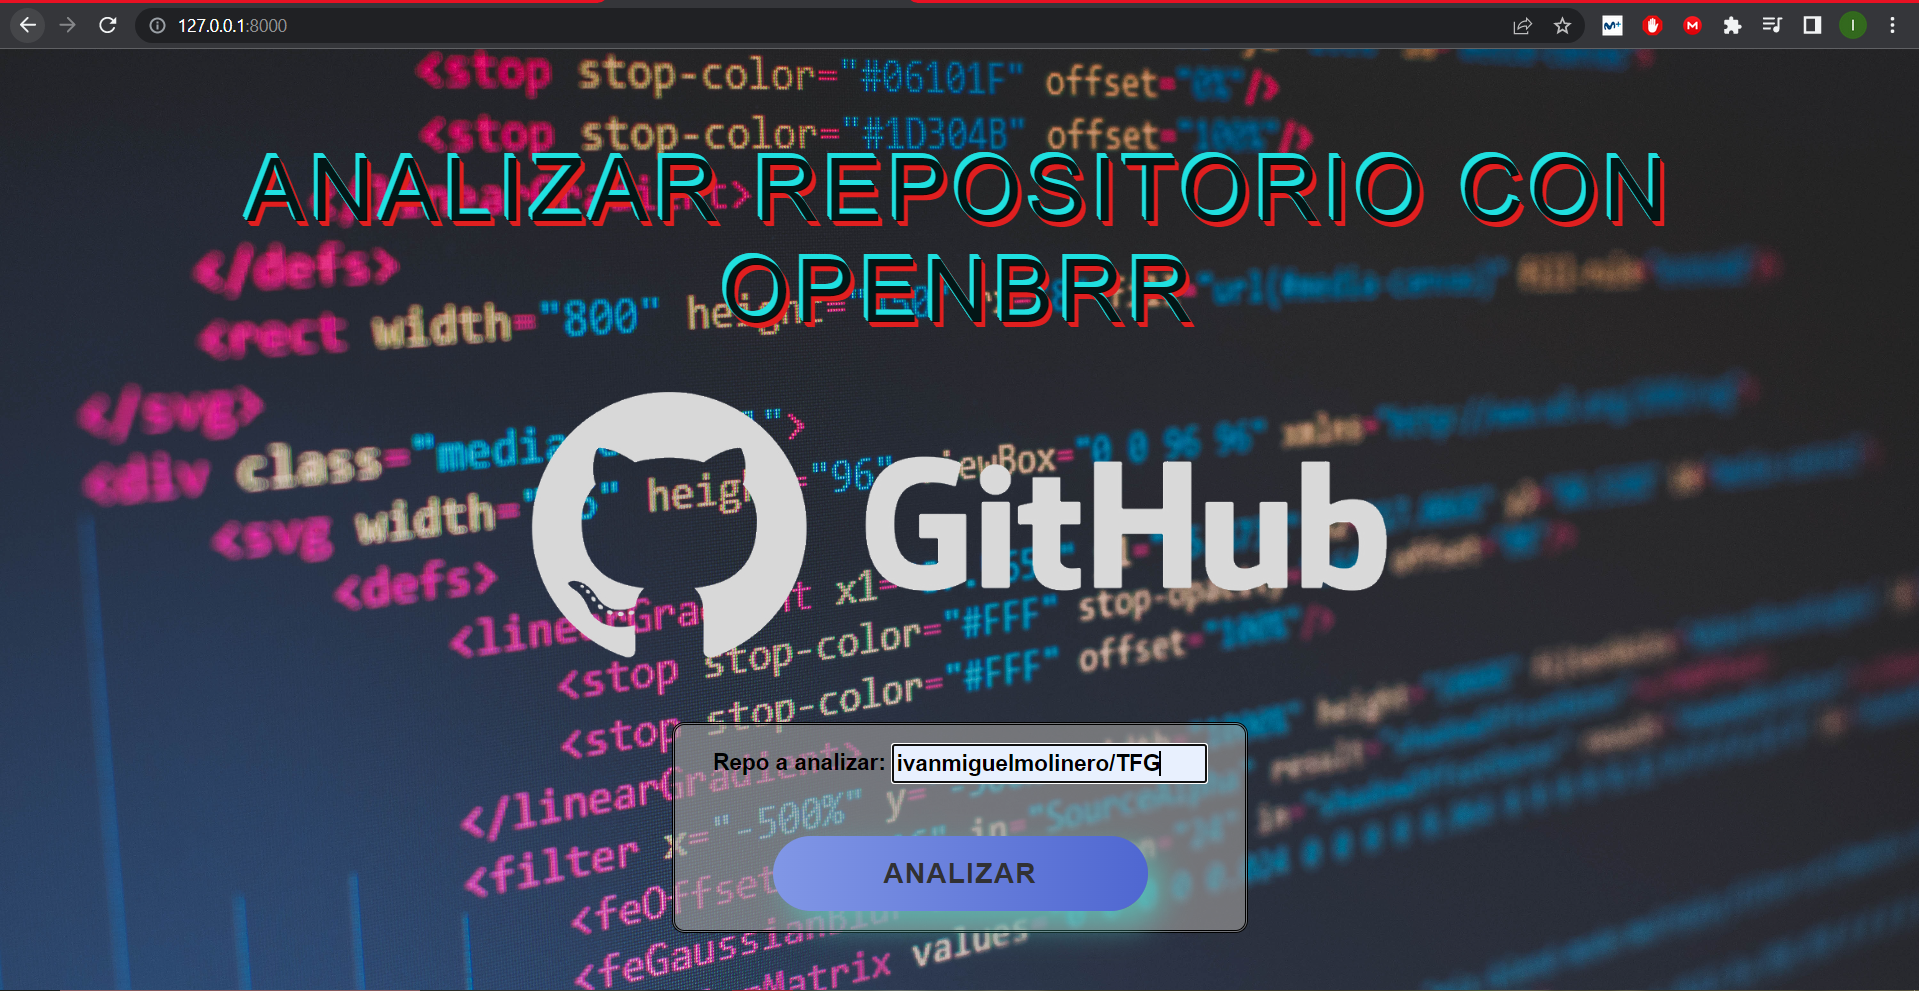
\includegraphics[bb=0 0 800 600, width=12cm, keepaspectratio]{img/maintfg.png}
    \caption{Página principal con el formulario relleno}\label{fig:ivanmiguelmolinero/TFG}
\end{figure}

A continuación se pasan a explicar cada uno de los ficheros de importancia de Django.

\subsubsection{urls.py}

Es el fichero encargado de gestionar las peticiones que le llegan comunicándose con views.py. El usuario lanza una petición y, en función de esta, este fichero activa una función u otra de views.py. Por ejemplo, si el usuario introduce la dirección raíz, urls.py se encarga de que se acabe mostrando la página principal mediante la función views.post\textunderscore main. Las otras dos URLS que debe gestionar se corresponden con el envío del formulario de la página principal (figura~\ref{fig:ivanmiguelmolinero/TFG}) y el envío del formulario de repo\textunderscore data.html

\subsubsection{forms.py}

Fichero que define el modelo de formulario a utilizar

\subsubsection{models.py}

Fichero que da forma al modelo definido en forms.py

\subsubsection{settings.py}

Este es el fichero de configuración de Django, en él se deben especificar:

\begin{itemize}
	\item Directorio donde está guardado el fichero credentials.py correspondiente a las credenciales de Gmail necesarias para el envío del correo.
	\item Directorio base a partir del cual funcionará la aplicación.
	\item Clave secreta.
	\item Hosts permitidos: en este caso son 127.0.0.0 (localhost) y pythonanywhere.com.
	\item Las apps instaladas en el sitio.
	\item La lógica de intercambio de información o middleware\cite{website:middleware}.
	\item La definición de las plantillas.
	\item La base de datos donde se guardarían diferentes valores si se necesitara.
	\item El idioma del lenguaje.
	\item La zona horaria.
	\item La URL y el directorio raíz.
	\item Los valores necesarios para el envío del correo: EMAIL\textunderscore BACKEND, EMAIL\textunderscore HOST, EMAIL\textunderscore USE\textunderscore TLS, EMAIL\textunderscore PORT, EMAIL\textunderscore HOST\textunderscore USER y EMAIL\textunderscore HOST\textunderscore PASSWORD.
\end{itemize}

\subsubsection{manage.py}

Es el fichero encargado de iniciar el servidor como se indica en el manual de usuario y gestionar el error de no haber instalado correctamente Django. Función mediante el siguiente comando:

\begin{verbatim}
	python manage.py runserver
\end{verbatim}

\subsection{Javascript}

Los ficheros javascript son los encargados de la interacción aplicación-usuario. En el caso de esta aplicación, la plantilla repo\textunderscore data.html funciona gracias al fichero datos.js

\subsubsection{datos.js}

Controla que el usuario pueda ocultar y mostrar las pestañas de los parámetros de OpenBRR, controla que no pueda introducir valores superiores al 100\% (función edit\textunderscore max\textunderscore value\textunderscore [parámetro] y get\textunderscore suma) y que pueda modificar los datos mostrados (función save\textunderscore input\textunderscore [parámetro]). Además, controla que solo pueda enviar el formulario si se están mostrando para evitar el error de enviar el formulario vacío.

\subsection{Plantillas HTML}

Es lo que se muestra al usuario una vez renderizadas. La aplicación cuenta con las siguientes:

\begin{itemize}
	\item \textbf{Main.html:} Correspondiente a la página principal muestra el nombre de la aplicación y el formulario para enviar el nombre del repositorio a analizar.
	\item \textbf{Repo\textunderscore data.html:} Muestra los datos del repositorio en diferentes pestañas que el usuario puede mostrar u ocultar. También puede modificar esos datos. Al final hay un formulario para introducir su dirección de correo donde recibirá los resultados de su análisis.
	\item \textbf{Result.html:} Muestra la calificación final de cada uno de los parámetros y del repositorio.
	\item \textbf{Error.html:} Página que se muestra si el repositorio introducido no existe. Permite al usuario volver a la página principal.
	\item \textbf{Overflow.html:} Página que se muestra cuando se excede el número de peticiones a Github. Permite al usuario volver a la página principal.
\end{itemize}

\subsection{Ficheros CSS}

Son los que dan estilo a cada una de las plantillas HTML.

\subsection{Ejemplo de uso}

De la figura~\ref{fig:ivanmiguelmolinero/TFG} a la figura~\ref{fig:resultados_3} tenemos un ejemplo analizando el repositorio de este TFG.

\begin{figure}
    
    \includegraphics[bb=0 0 800 600, width=12cm, keepaspectratio]{img/pestañas_off.png}
    \caption{Página de datos con las pestañas ocultas.}\label{fig:pestañas_off}
\end{figure}

\begin{figure}
    
    \includegraphics[bb=0 0 800 600, width=12cm, keepaspectratio]{img/pestañas_1.png}
    \caption{Primera parte de la página de datos.}\label{fig:pestañas_1}
\end{figure}

\begin{figure}
    
    \includegraphics[bb=0 0 800 600, width=12cm, keepaspectratio]{img/pestañas_2.png}
    \caption{Segunda parte de la página de datos.}\label{fig:pestañas_2}
\end{figure}

\begin{figure}
    
    \includegraphics[bb=0 0 800 600, width=12cm, keepaspectratio]{img/pestañas_3.png}
    \caption{Tercera parte de la página de datos.}\label{fig:pestañas_3}
\end{figure}

\begin{figure}
    
    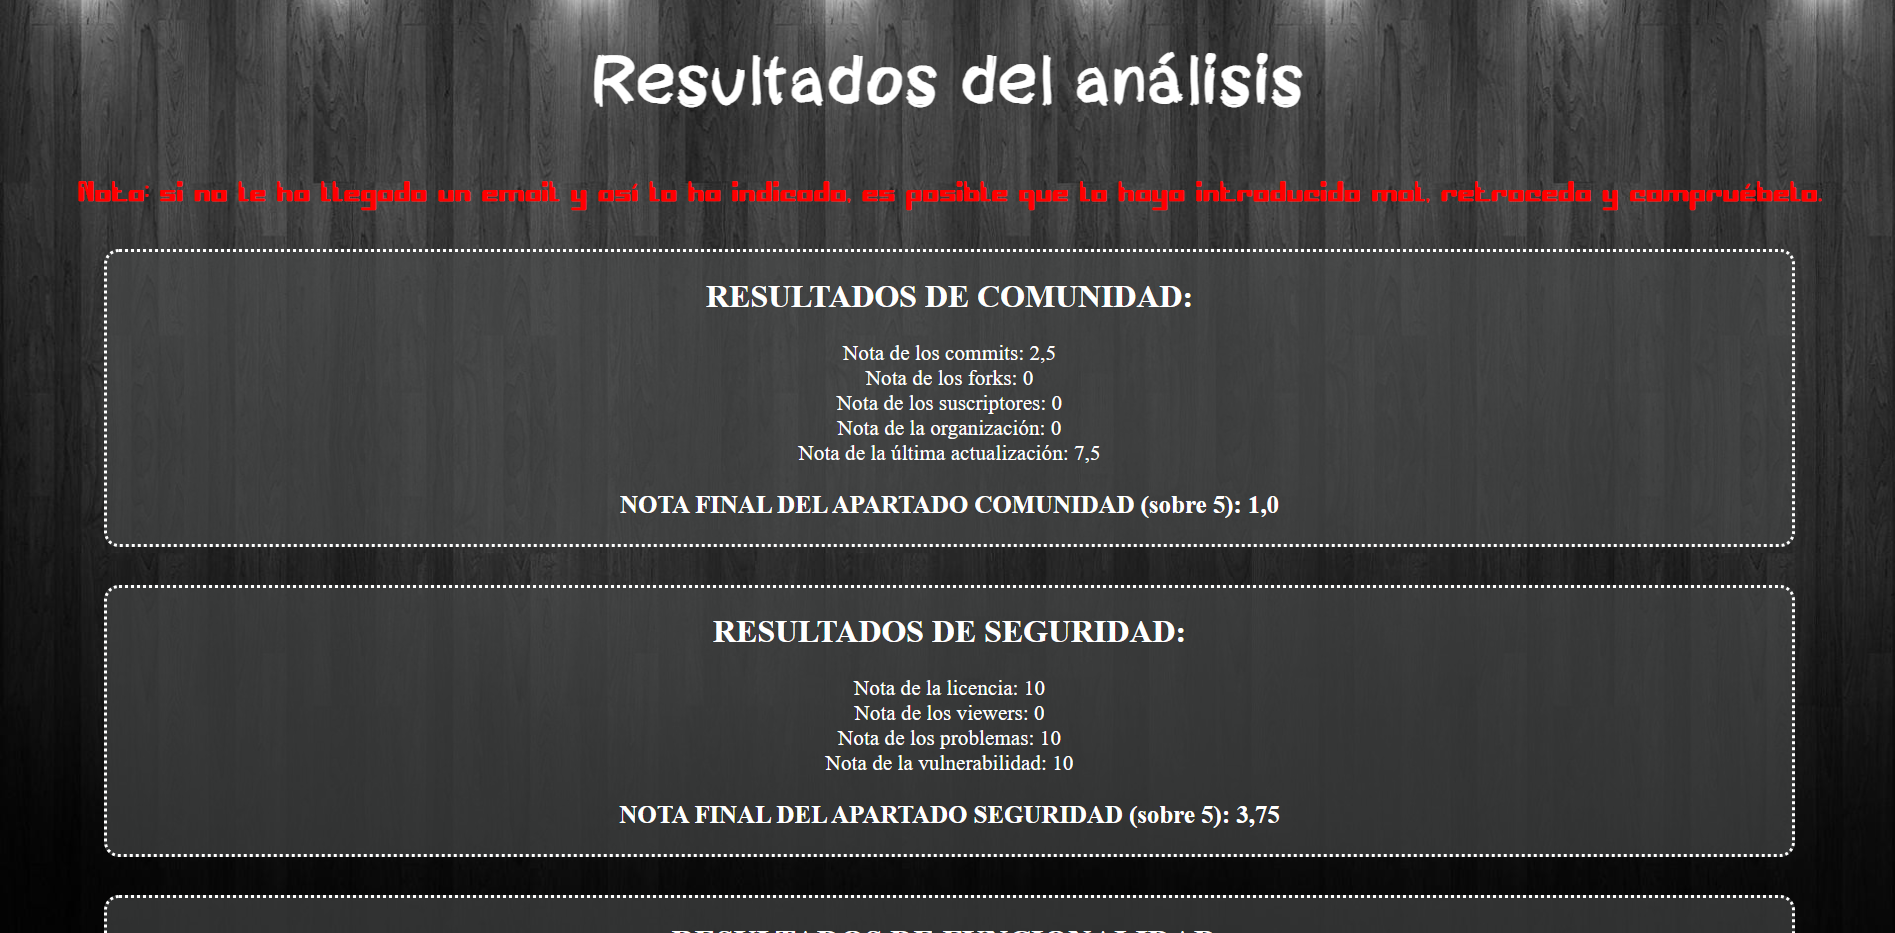
\includegraphics[bb=0 0 800 600, width=12cm, keepaspectratio]{img/resultados_1.png}
    \caption{Primera parte de la página de resultados.}\label{fig:resultados_1}
\end{figure}

\begin{figure}
    
    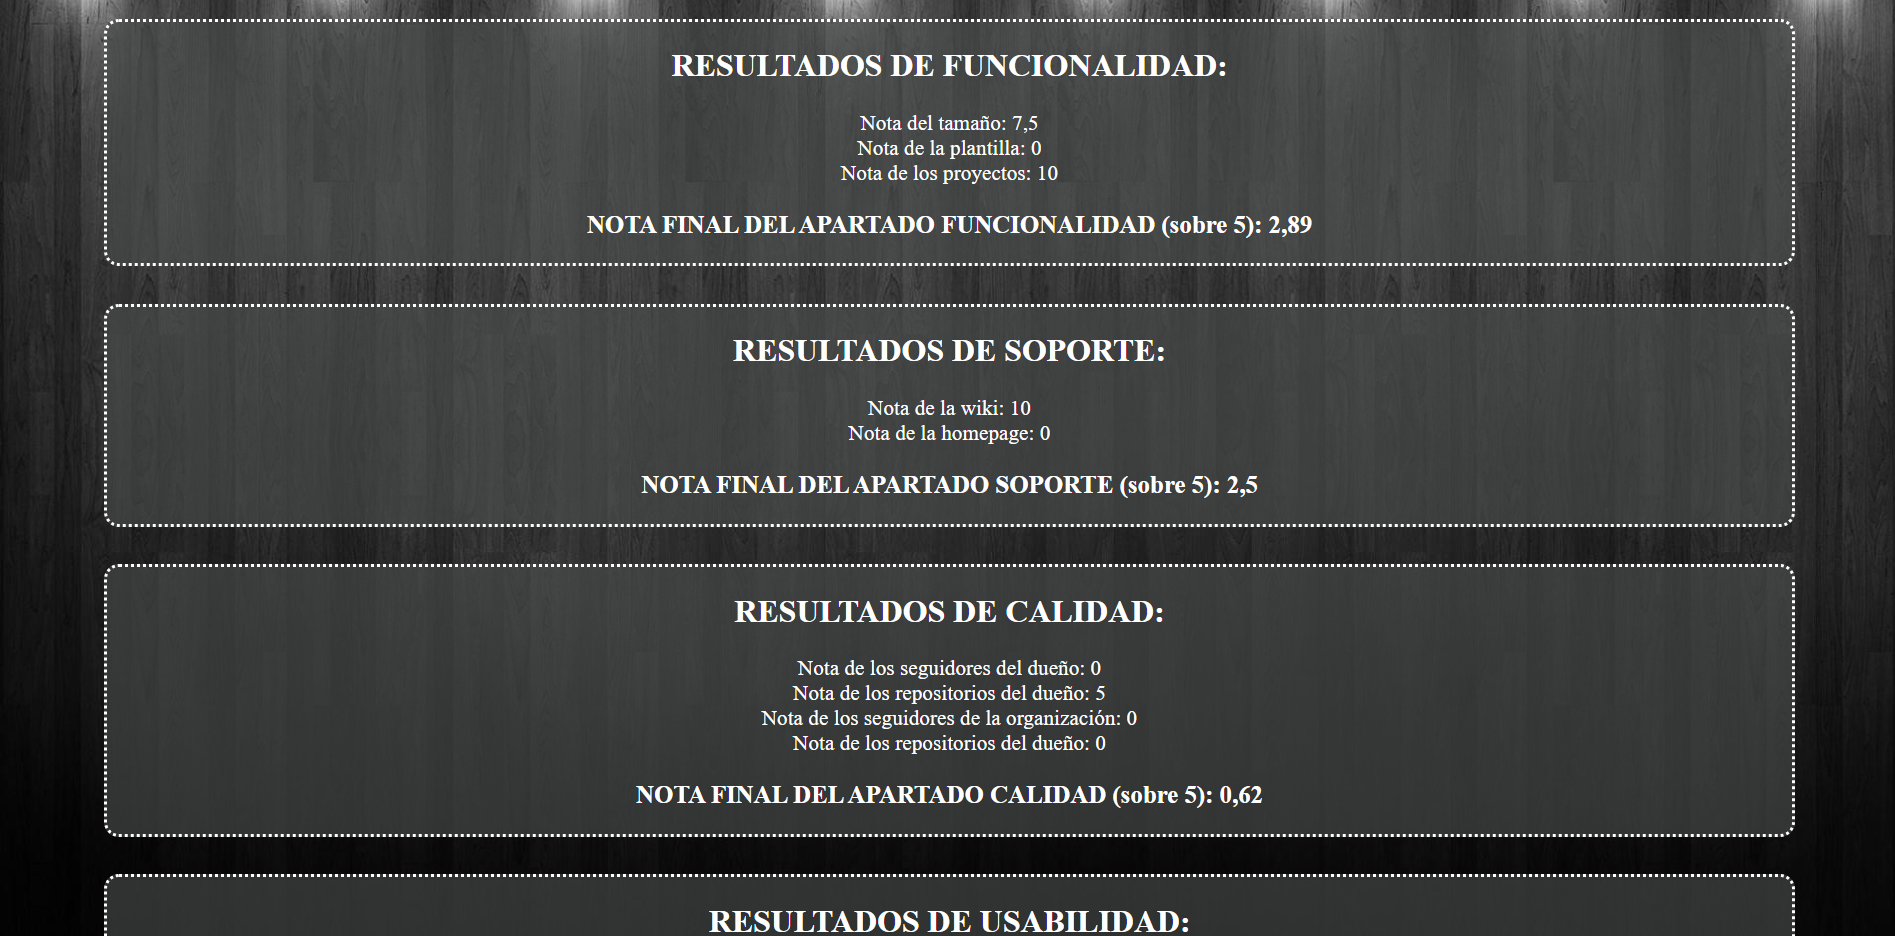
\includegraphics[bb=0 0 800 600, width=12cm, keepaspectratio]{img/resultados_2.png}
    \caption{Segunda parte de la página de resultados.}\label{fig:resultados_2}
\end{figure}

\begin{figure}
    
    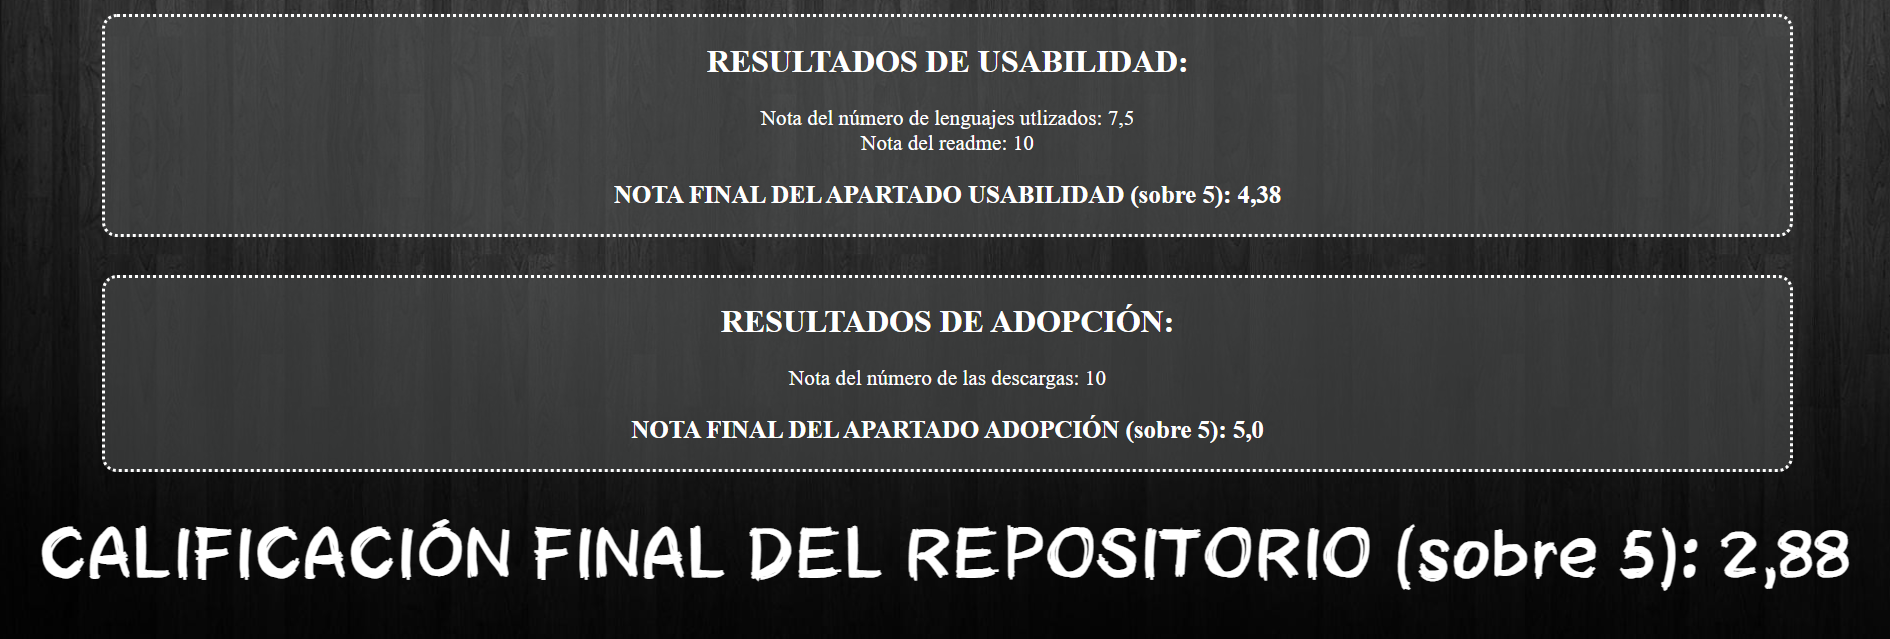
\includegraphics[bb=0 0 800 600, width=12cm, keepaspectratio]{img/resultados_3.png}
    \caption{Tercera parte de la página de resultados.}\label{fig:resultados_3}
\end{figure}


%%%%%%%%%%%%%%%%%%%%%%%%%%%%%%%%%%%%%%%%%%%%%%%%%%%%%%%%%%%%%%%%%%%%%%%%%%%%%%%%
%%%%%%%%%%%%%%%%%%%%%%%%%%%%%%%%%%%%%%%%%%%%%%%%%%%%%%%%%%%%%%%%%%%%%%%%%%%%%%%%
% EXPERIMENTOS Y VALIDACIÓN %
%%%%%%%%%%%%%%%%%%%%%%%%%%%%%%%%%%%%%%%%%%%%%%%%%%%%%%%%%%%%%%%%%%%%%%%%%%%%%%%%

\cleardoublepage
\chapter{Experimentos y validación}
\label{chap:experimentos}

En este capítulo se explicarán las diferentes pruebas que se fueron haciendo durante el desarrollo de este proyectos con los diferentes paquetes y frameworks.

\section{Perceval}

Esta fue la librería propuesta inicialmente por mi tutor. Realicé varias pruebas siguiendo los pasos indicados en su página\footnote{\url{https://perceval.readthedocs.io/en/latest/perceval/git.html#using-perceval-as-a-python-module}} pero debido a su complejidad y que solo conseguía que funcionara en Linux\footnote{\url{https://www.linux.org/}} se terminó descartando en favor de PyGithub. En la figura~\ref{fig:perceval} podemos observar un programa de prueba con Perceval que extraía los ''pull request'' y los ''issues'' de un repositorio.

\begin{figure}
    \centering
    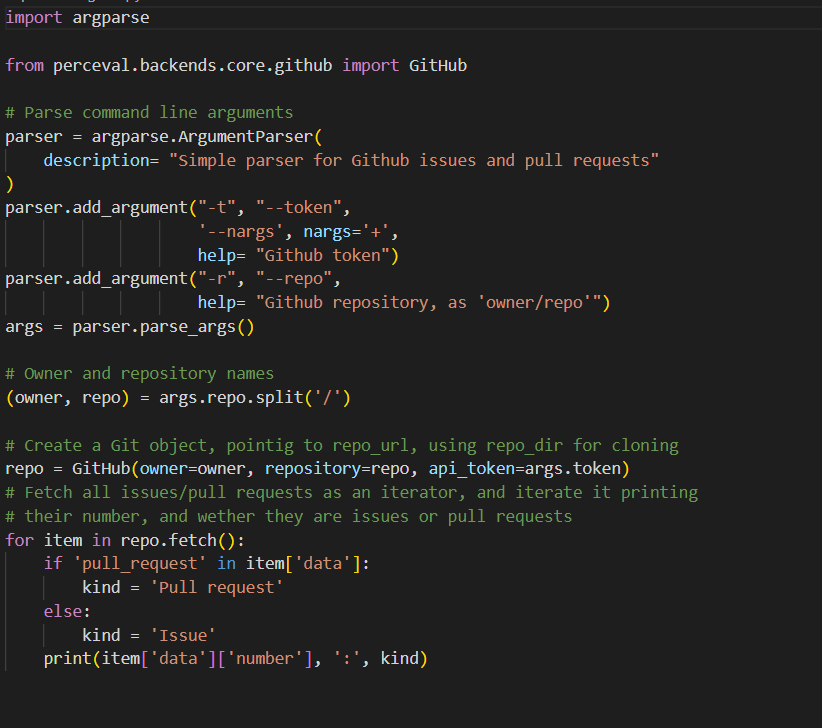
\includegraphics[width=1\textwidth, keepaspectratio]{img/perceval.png}
    \caption{Programa de prueba de Perceval.}\label{fig:perceval}
\end{figure}

\section{PyGithub}

Por los motivos explicados anteriormente se descartó Perceval y se reemplazó por PyGithub. Al principio, se hicieron diferentes pruebas con diferentes funciones de esta librería para comprobar su correcto funcionamiento antes de implementarla en la aplicación final. Se seleccionó como repositorio de pruebas el propio de PyGithub\footnote{\url{https://github.com/pygithub/pygithub}} y se extrajeron diferentes datos que fueran fácilmente comprobables desde la página de Github. De la figura~\ref{fig:pygithub_1} a la figura~\ref{fig:pestañas_3} podemos ver el programa de prueba resultante y en la figura~\ref{fig:pygithub_salida} su salida. Finalmente, de la figura~\ref{fig:pygithub_commits} a la figura~\ref{fig:pygithub_lenguajes} observamos los datos mostrados por el propio repositorio y comprobamos que se corresponden con los obtenidos por la salida del programa de prueba. Por tanto, el programa funciona correctamente.

\begin{figure}
    \centering
    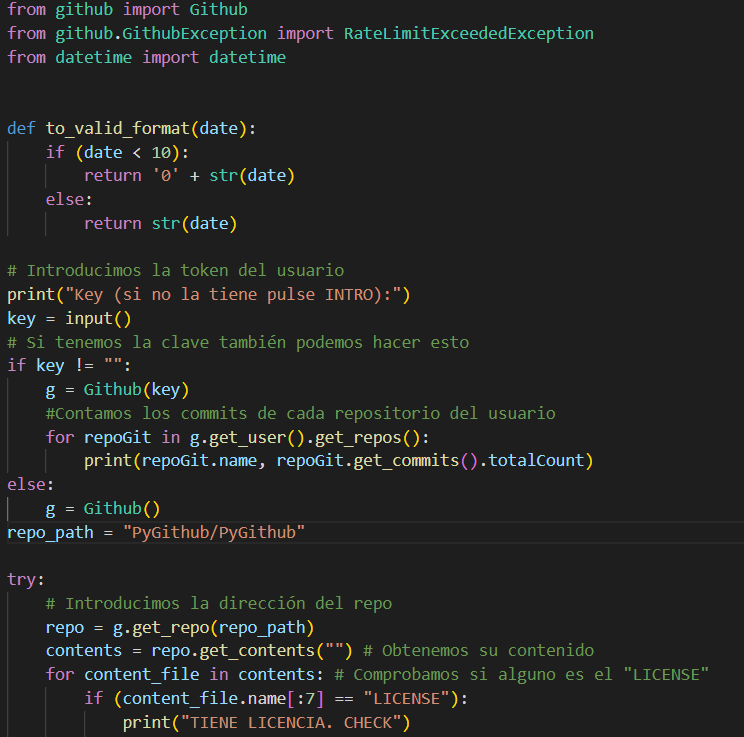
\includegraphics[width=1\textwidth, keepaspectratio]{img/pygithub_1.png}
    \caption{Primera parte del programa de prueba de PyGithub.}\label{fig:pygithub_1}
\end{figure}

\begin{figure}
    \centering
    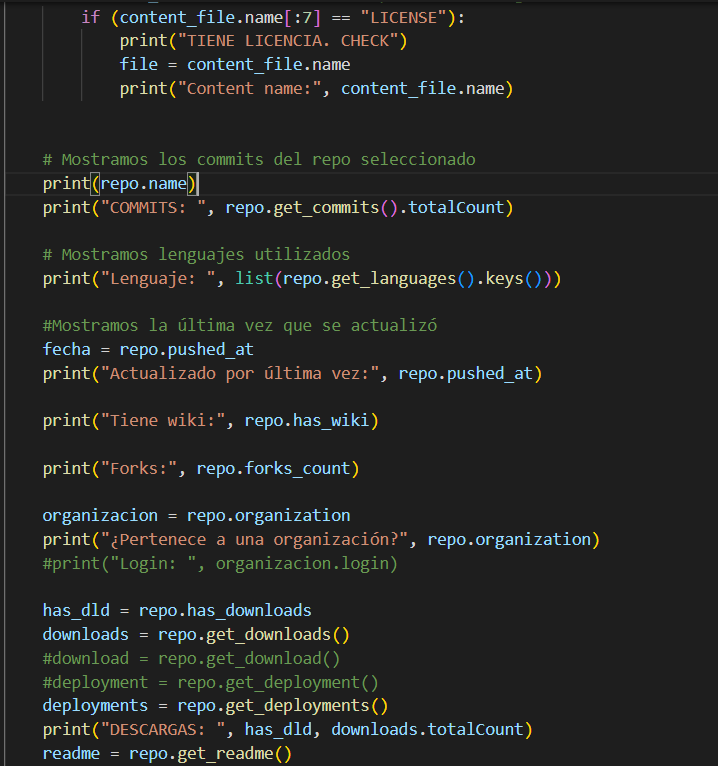
\includegraphics[width=1\textwidth, keepaspectratio]{img/pygithub_2.png}
    \caption{Segunda parte del programa de prueba de PyGithub.}\label{fig:pygithub_2}
\end{figure}
  
\begin{figure}
    \centering
    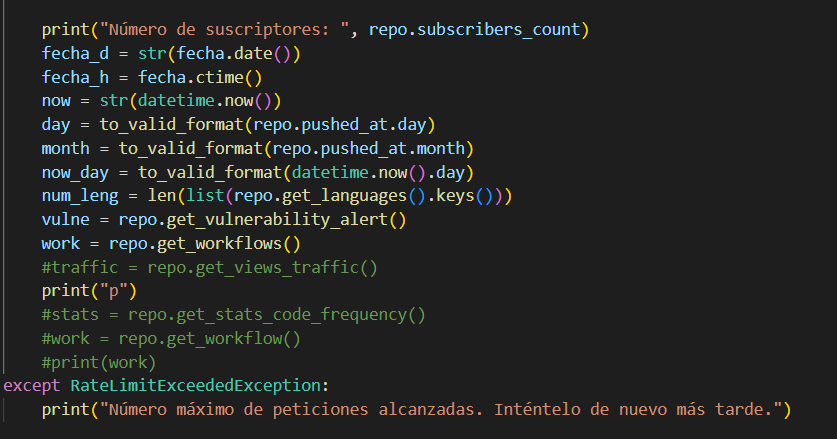
\includegraphics[width=1\textwidth, keepaspectratio]{img/pygithub_3.png}
    \caption{Tercera parte del programa de prueba de PyGithub.}\label{fig:pygithub_3}
\end{figure}

\begin{figure}
    \centering
    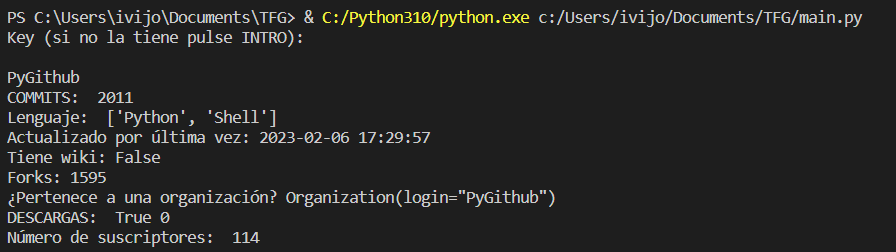
\includegraphics[width=1\textwidth, keepaspectratio]{img/pygithub_salida.png}
    \caption{Salida del programa de prueba de PyGithub.}\label{fig:pygithub_salida}
\end{figure}

\begin{figure}
    \centering
    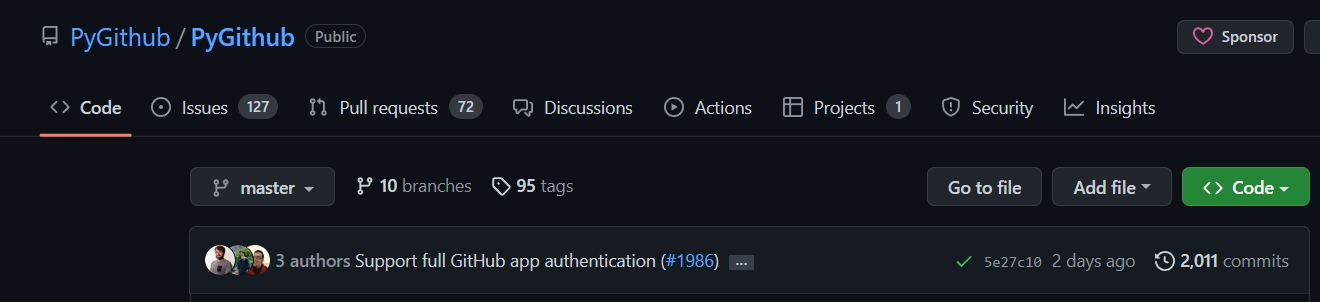
\includegraphics[width=1\textwidth, keepaspectratio]{img/pygithub_commits.png}
    \caption{Número de commits de PyGithub.}\label{fig:pygithub_commits}
\end{figure}

\begin{figure}
    \centering
    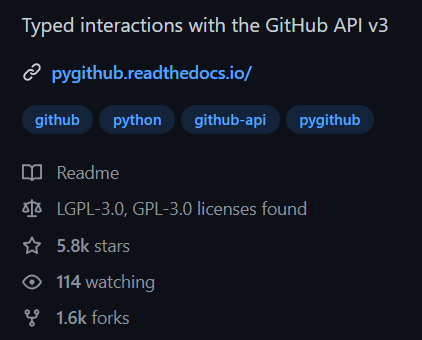
\includegraphics[width=1\textwidth, keepaspectratio]{img/pygithub_forks.png}
    \caption{Número de forks de PyGithub.}\label{fig:pygithub_forks}
\end{figure}

\begin{figure}
    \centering
    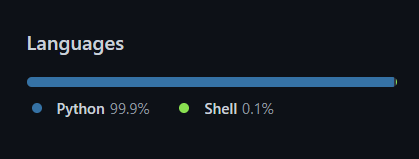
\includegraphics[width=1\textwidth, keepaspectratio]{img/pygithub_lenguajes.png}
    \caption{Lenguajes utilizados en el repositorio de PyGithub.}\label{fig:pygithub_lenguajes}
\end{figure}

\section{Pruebas con la aplicación}

Una vez comprobado el correcto funcionamiento de PyGithub, se implementa en la aplicación junto con Django. Para corroborar que las peticiones se envían y el repositorio se analiza correctamente, rellenamos el formulario inicial con el repositorio de PyGithub (como en el apartado anterior) para ver si los datos obtenidos coinciden. La página principal queda tal y como observamos en la figura~\ref{fig:pricipal_pygithub}. Finalmente, en la ventana de datos que podemos ver en la figura~\ref{fig:comunidad_pygithub} observamos que los datos obtenidos coinciden con los obtenidos en la figura~\ref{fig:pygithub_salida} y que, por tanto, la implementación ha sido un éxito.

\subsection{Pruebas con views.py}

Como se ha explicado en el apartado~\ref{sec:views.py} este fichero es muy importante para el correcto funcionamiento de la aplicación, por ello es de vital importancia asegurarse de que funciona perfectamente. Debido a su extensión, se explicarán las pruebas que se hicieron poniendo de ejemplo la pestaña comunidad de la figura~\ref{fig:comunidad_pygithub} y se darán por explicadas todas las demás ya que, además, su funcionamiento es exactamente el mismo.

Views.py se encarga, entre otras muchas cosas, de recoger los datos enviados por el usuario en el formulario y obtener la calificación de cada apartado y la calificación final del repositorio. Para la pestaña comunidad, como no se han modificado los valores de la aportación de cada dato, se obtiene su calificación final sobre 5 con la siguiente fórmula:

\begin{verbatim}
nota final = (nota commits * 0.2 + nota forks * 0.2
+ nota suscriptores * 0.2 + nota organización * 0.2 
+ nota actualización * 0.2)/2
\end{verbatim}

Para el cálculo de la calificación de cada dato en concreto se usan los métodos que podemos ver de la figura~\ref{fig:nota_commits} a la figura~\ref{fig:nota_actualización} en función del número introducido por el usuario en el formulario de la figura~\ref{fig:comunidad_pygithub}. Cabe destacar que, en caso de tratarse de un formulario de ''sí o no'' la nota es binaria, es decir, un 10 si cumple el requisito o un 0 si no lo cumple. Esto lo podemos ver en la figura~\ref{fig:nota_organización}.

Si obtenemos la nota final a mano obtenemos que la nota de cada apartado es:

\begin{verbatim}
nota commits = 10
nota forks = 10
nota suscriptores = 10
nota organización = 10
nota actualización = 7.5
\end{verbatim}

Por tanto, aplicando la fórmula anterior obtenemos una calificación de 4.75 que es lo mismo que ha calculado la aplicación como vemos en la figura~\ref{fig:test_comunidad} así que funciona correctamente. Por último, comprobamos que obtiene de manera correcta la nota media de todos los apartados. A mano, calculamos la nota final sumando las notas de cada apartado, que podemos observar de la figura~\ref{fig:test_comunidad} a la figura~\ref{fig:test_adopción_y_notafinal} y dividiendo entre 7 para obtener una nota final de:

\begin{verbatim}
nota final = (4.75 + 4.38 + 2.06 + 2.5 + 0 + 5 + 5)/ 7 = 3.38
\end{verbatim}

Como vemos en esta última figura, la aplicación ha calculado la nota correctamente y podemos concluir que funciona.

\begin{figure}
    \centering
    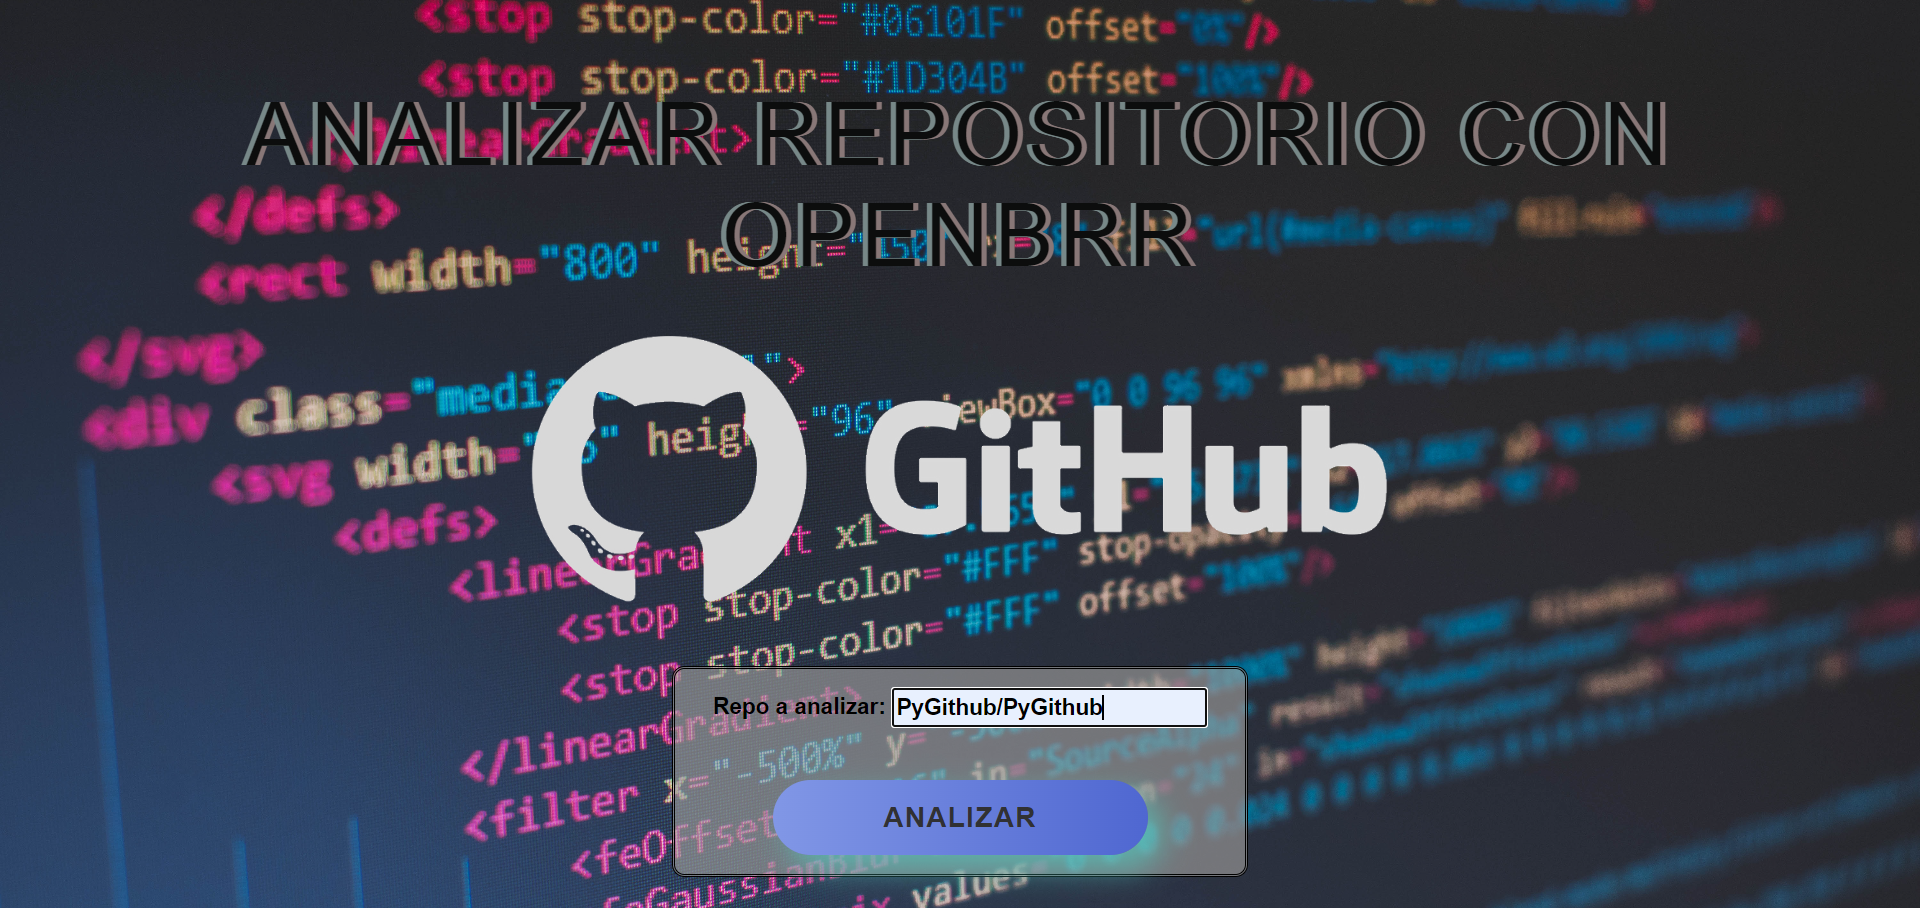
\includegraphics[width=1\textwidth, keepaspectratio]{img/principal_main.png}
    \caption{Página principal antes de analizar PyGithub.}\label{fig:pricipal_pygithub}
\end{figure}

\begin{figure}
    \centering
    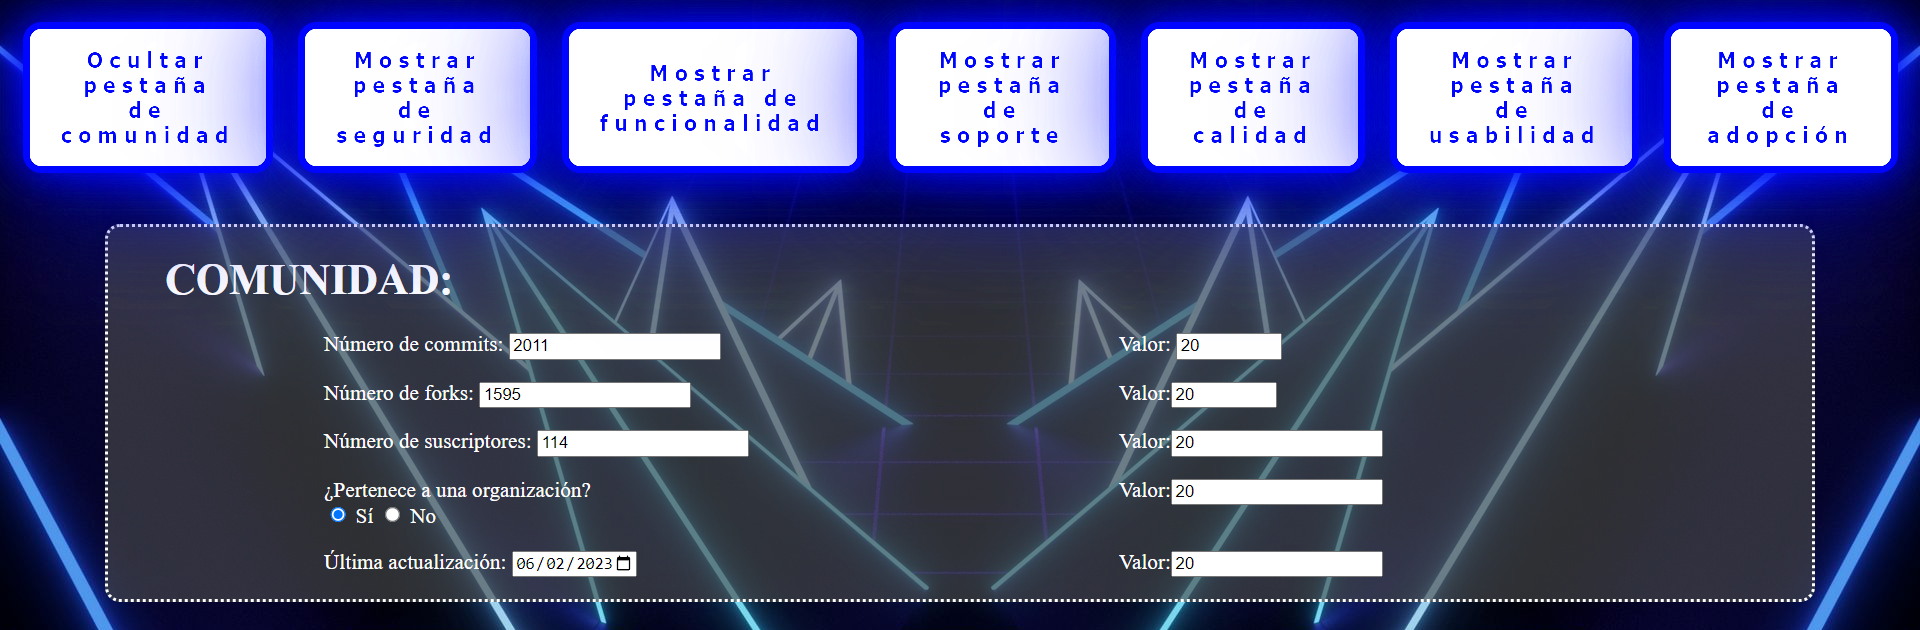
\includegraphics[width=1\textwidth, keepaspectratio]{img/pygithub_comunidad.png}
    \caption{Pestaña de comunidad de PyGithub.}\label{fig:comunidad_pygithub}
\end{figure}

\begin{figure}
    \centering
    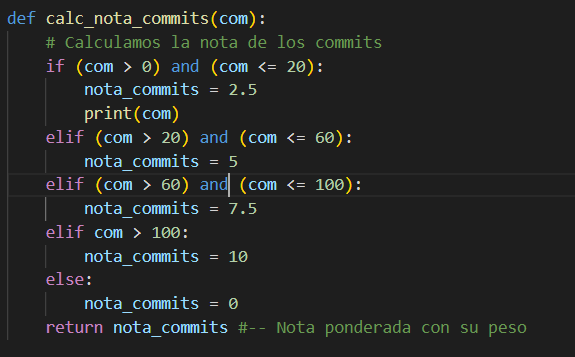
\includegraphics[width=1\textwidth, keepaspectratio]{img/nota_commits.png}
    \caption{Obtención de la calificación en función del número de commits.}\label{fig:nota_commits}
\end{figure}

\begin{figure}
    \centering
    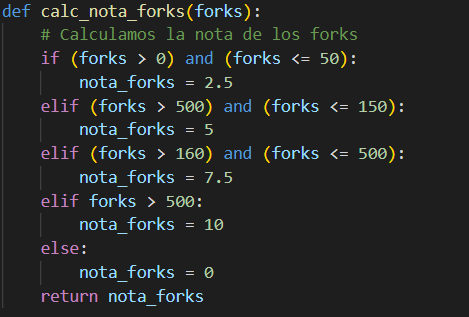
\includegraphics[width=1\textwidth, keepaspectratio]{img/nota_forks.png}
    \caption{Obtención de la calificación en función del número de forks.}\label{fig:nota_forks}
\end{figure}

\begin{figure}
    \centering
    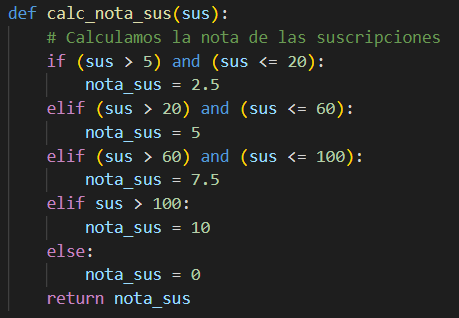
\includegraphics[width=1\textwidth, keepaspectratio]{img/nota_suscriptores.png}
    \caption{Obtención de la calificación en función del número de suscriptores.}\label{fig:nota_suscriptores}
\end{figure}

\begin{figure}
    \centering
    \includegraphics[width=1\textwidth, keepaspectratio]{img/nota_organización.png}
    \caption{Obtención de la calificación en función de si pertenece a una organización.}\label{fig:nota_organización}
\end{figure}

\begin{figure}
    \centering
    \includegraphics[width=1\textwidth, keepaspectratio]{img/nota_actualización.png}
    \caption{Obtención de la calificación en función de la fecha de última actualización.}\label{fig:nota_actualización}
\end{figure}

\begin{figure}
    \centering
    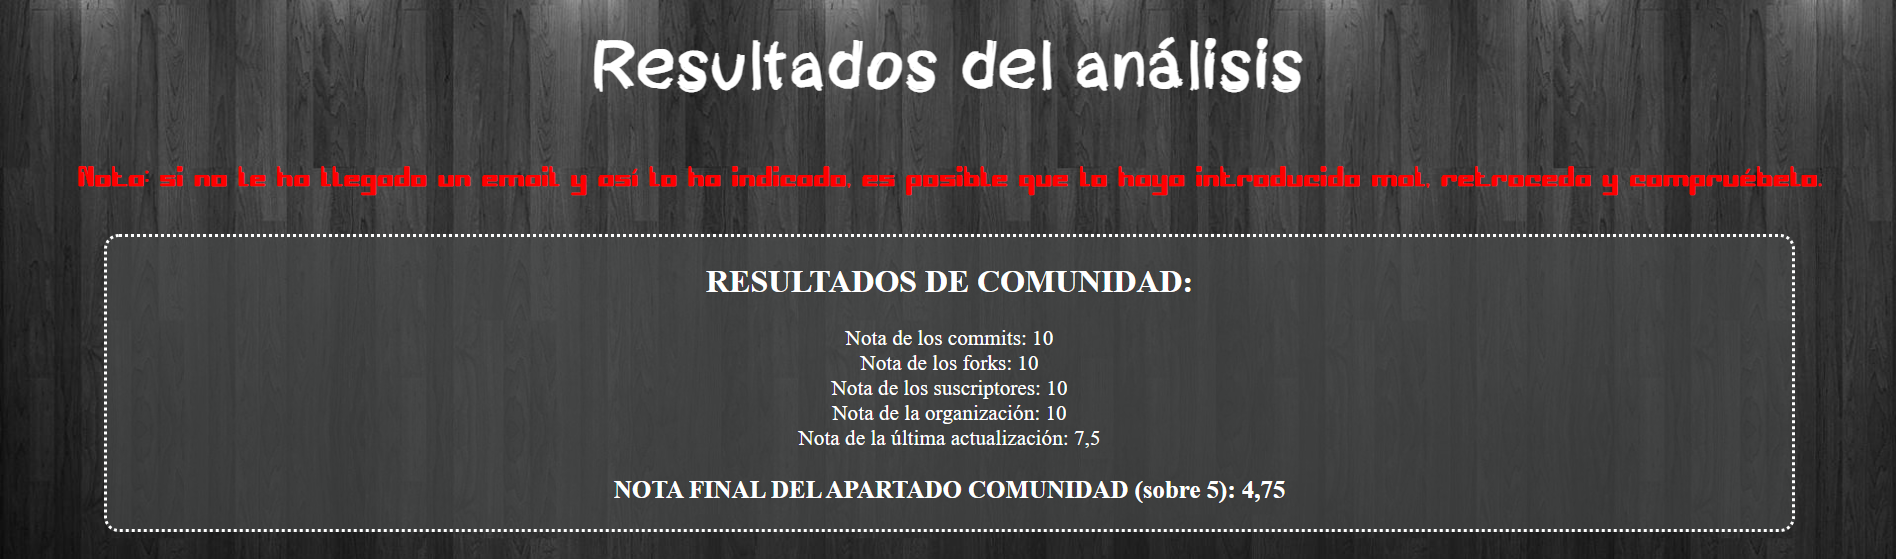
\includegraphics[width=1\textwidth, keepaspectratio]{img/test_comunidad.png}
    \caption{Calificación de comunidad obtenida por la aplicación.}\label{fig:test_comunidad}
\end{figure}

\begin{figure}
    \centering
    
\includegraphics[width=1\textwidth, keepaspectratio]{img/test_seguridad.png}
    \caption{Calificación de seguridad obtenida por la aplicación.}\label{fig:test_seguridad}
\end{figure}

\begin{figure}
    \centering
    
\includegraphics[width=1\textwidth, keepaspectratio]{img/test_funcionalidad.png}
    \caption{Calificación de funcionalidad obtenida por la aplicación.}\label{fig:test_funcionalidad}
\end{figure}

\begin{figure}
    \centering
    
\includegraphics[width=1\textwidth, keepaspectratio]{img/test_soporte.png}
    \caption{Calificación de soporte obtenida por la aplicación.}\label{fig:test_soporte}
\end{figure}

\begin{figure}
    \centering
    
\includegraphics[width=1\textwidth, keepaspectratio]{img/test_calidad.png}
    \caption{Calificación de calidad obtenida por la aplicación.}\label{fig:test_calidad}
\end{figure}

\begin{figure}
    \centering
    
\includegraphics[width=1\textwidth, keepaspectratio]{img/test_usabilidad.png}
    \caption{Calificación de usabilidad obtenida por la aplicación.}\label{fig:test_usabilidad}
\end{figure}

\begin{figure}
    \centering
    \includegraphics[width=1\textwidth, keepaspectratio]{img/test_adopción_y_notafinal.png}
    \caption{Calificación de adopción y nota final obtenida por la aplicación.}\label{fig:test_adopción_y_notafinal}
\end{figure}

\subsubsection{Envío del correo}

Finalmente, el fichero views.py envía al usuario un mensaje a su dirección de correo que ha indicado con los mismos datos que podemos observar de la la figura~\ref{fig:test_comunidad} a la figura~\ref{fig:test_adopción_y_notafinal} por si quiere guardar ese análisis. Para comprobar su correcto funcionamiento indico mi dirección de correo en el formulario de la figura~\ref{fig:envio_correo}. Como podemos observar en la figura~\ref{fig:correo} los datos coinciden. El envío del correo es un éxito.

\begin{figure}
    \centering
    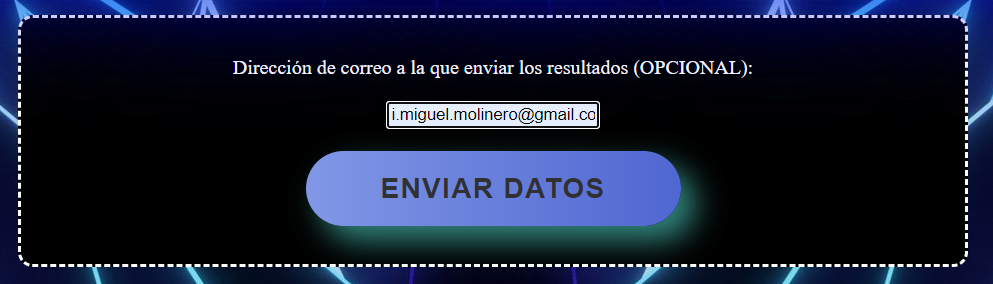
\includegraphics[width=1\textwidth, keepaspectratio]{img/envio_correo.png}
    \caption{Formulario rellenado con mi propia dirección de correo.}\label{fig:envio_correo}
\end{figure}

\begin{figure}
    \centering
    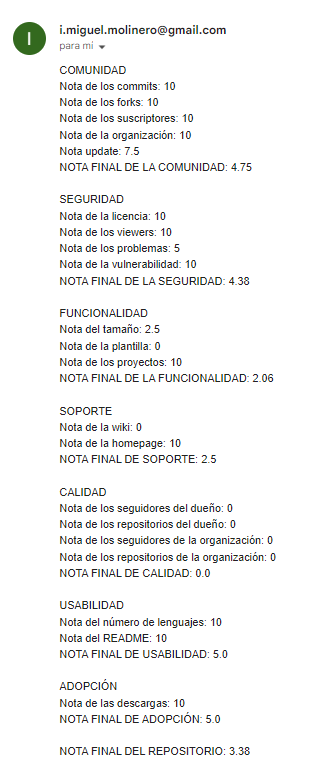
\includegraphics[ keepaspectratio]{img/correo.png}
    \caption{Mensaje enviado por la aplicación.}\label{fig:correo}
\end{figure}

%%%%%%%%%%%%%%%%%%%%%%%%%%%%%%%%%%%%%%%%%%%%%%%%%%%%%%%%%%%%%%%%%%%%%%%%%%%%%%%%
%%%%%%%%%%%%%%%%%%%%%%%%%%%%%%%%%%%%%%%%%%%%%%%%%%%%%%%%%%%%%%%%%%%%%%%%%%%%%%%%
% RESULTADOS %
%%%%%%%%%%%%%%%%%%%%%%%%%%%%%%%%%%%%%%%%%%%%%%%%%%%%%%%%%%%%%%%%%%%%%%%%%%%%%%%%

\cleardoublepage
\chapter{Resultados}
\label{chap:resultados}

Una vez hechas las pruebas explicadas en el capítulo~\ref{chap:experimentos} se pasa a comprobar que la aplicación devuelve resultados coherentes, es decir, que a repositorios teóricamente buenos les da una buena calificación y a repositorios prácticamente vacíos (como el de la prueba que se mostrará en el apartado~\ref{sec:vacio}) les da una mala calificación.

\section{Prueba con myTeachingURJC/Arq-computadores-01}

Este repositorio\footnote{\url{https://github.com/myTeachingURJC/Arq-computadores-01}}  es el de la asignatura ''Arquitectura de computadores'' de la URJC. A primera vista, como vemos en la figura~\ref{fig:myteachingURJC}, se podría decir que se trata de un buen repositorio. Vamos a analizarlo.

\begin{figure}
    \centering
    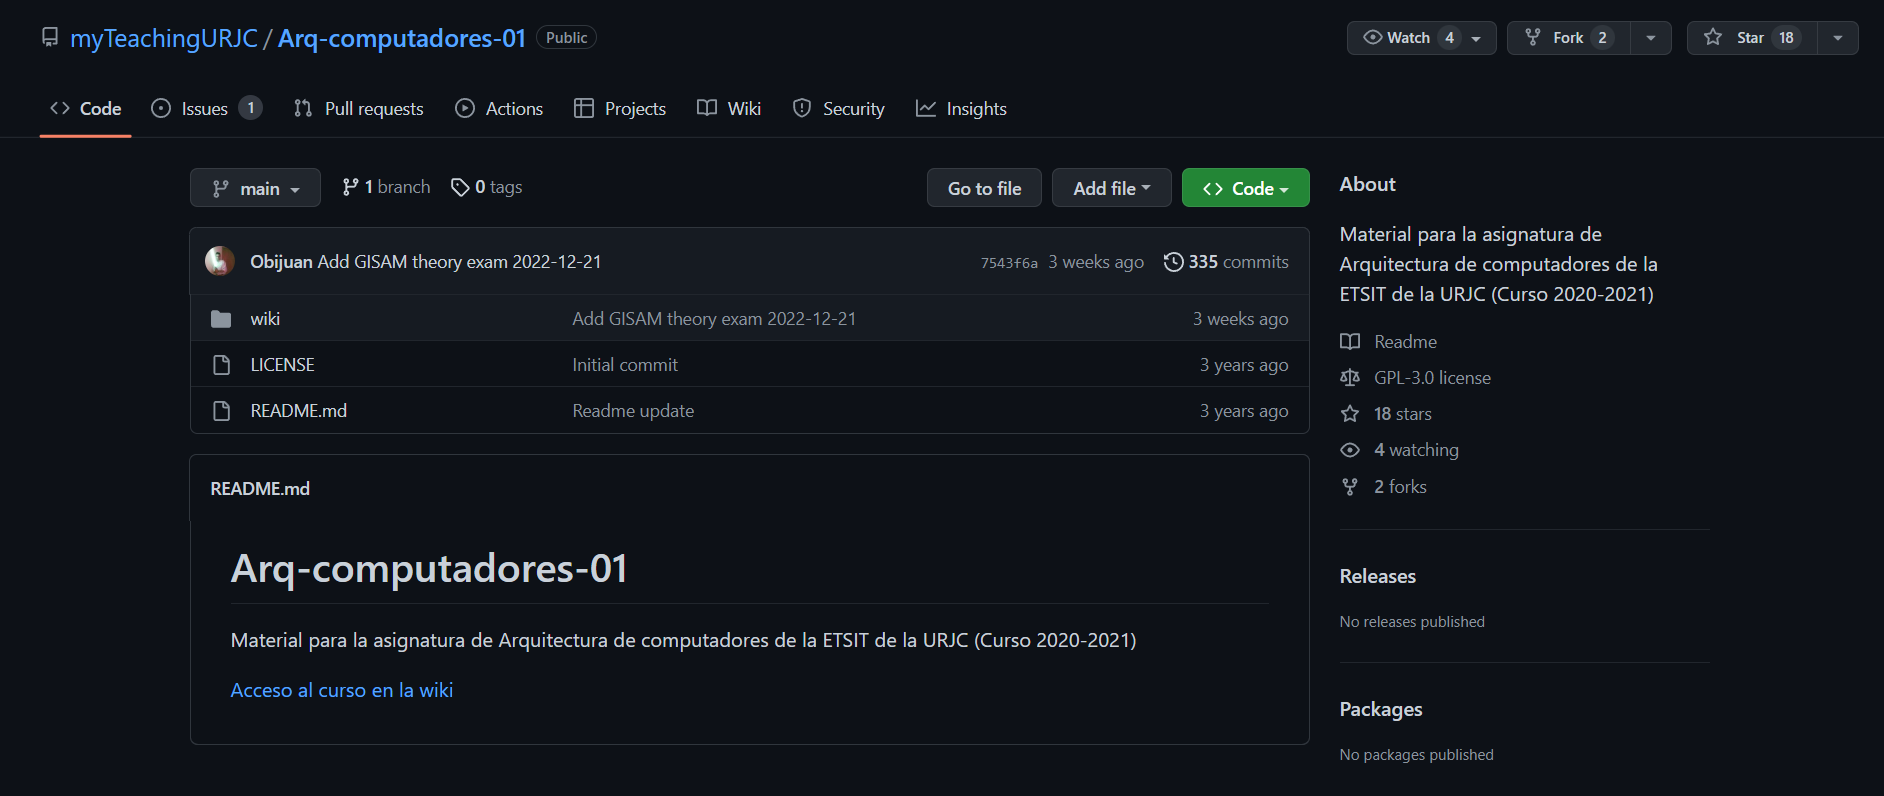
\includegraphics[ width=1.1\textwidth, keepaspectratio]{img/myteachingURJC.png}
    \caption{Vista inicial del repositorio de ''Arquitectura de computadores''.}\label{fig:myteachingURJC}
\end{figure}

\subsection{Análisis de myTeachingURJC/Arq-computadores-01}

De la figura~\ref{fig:myteachingURJC_1} a la figura ~\ref{fig:myteachingURJC_3} tenemos los datos del repositorio que vamos a mandar a través del formulario para su calificación. Como hemos visto en el capítulo~\ref{chap:experimentos}, los datos son correctos. 

\begin{figure}
    \centering
    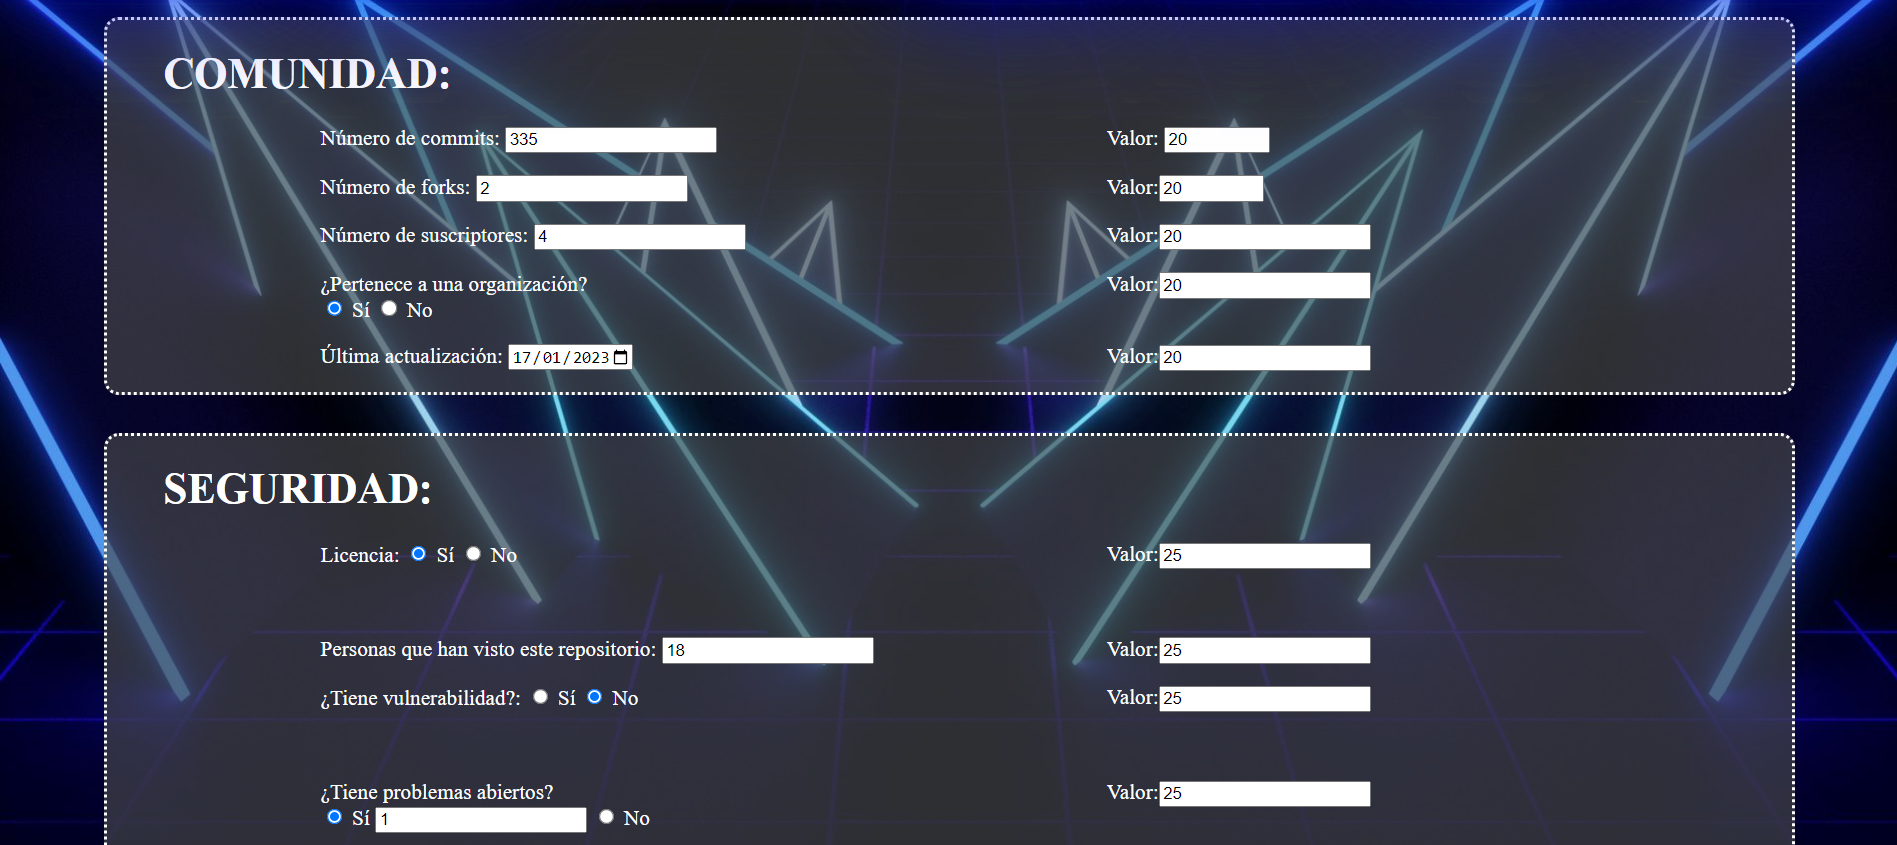
\includegraphics[ width=1.1\textwidth, keepaspectratio]{img/myteachingURJC_1.png}
    \caption{Datos del repositorio de ''Arquitectura de computadores''.}\label{fig:myteachingURJC_1}
\end{figure}

\begin{figure}
    \centering
    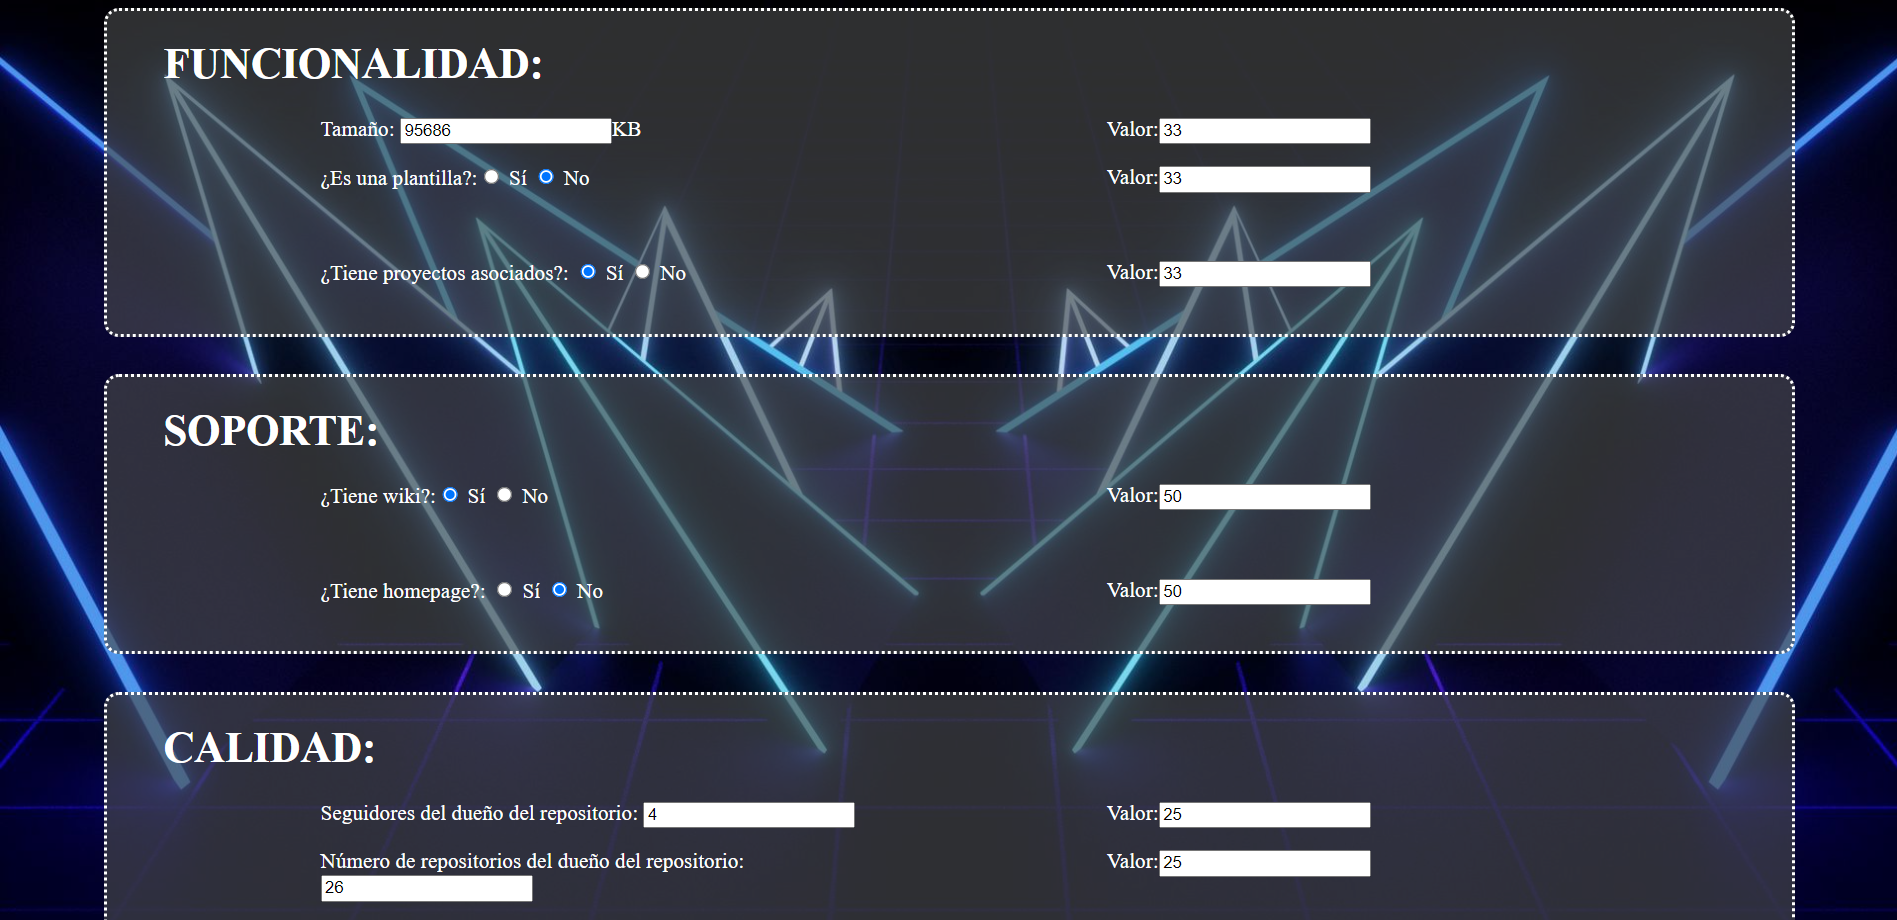
\includegraphics[ width=1.1\textwidth, keepaspectratio]{img/myteachingURJC_2.png}
    \caption{Datos del repositorio de ''Arquitectura de computadores''.}\label{fig:myteachingURJC_2}
\end{figure}

\begin{figure}
    \centering
    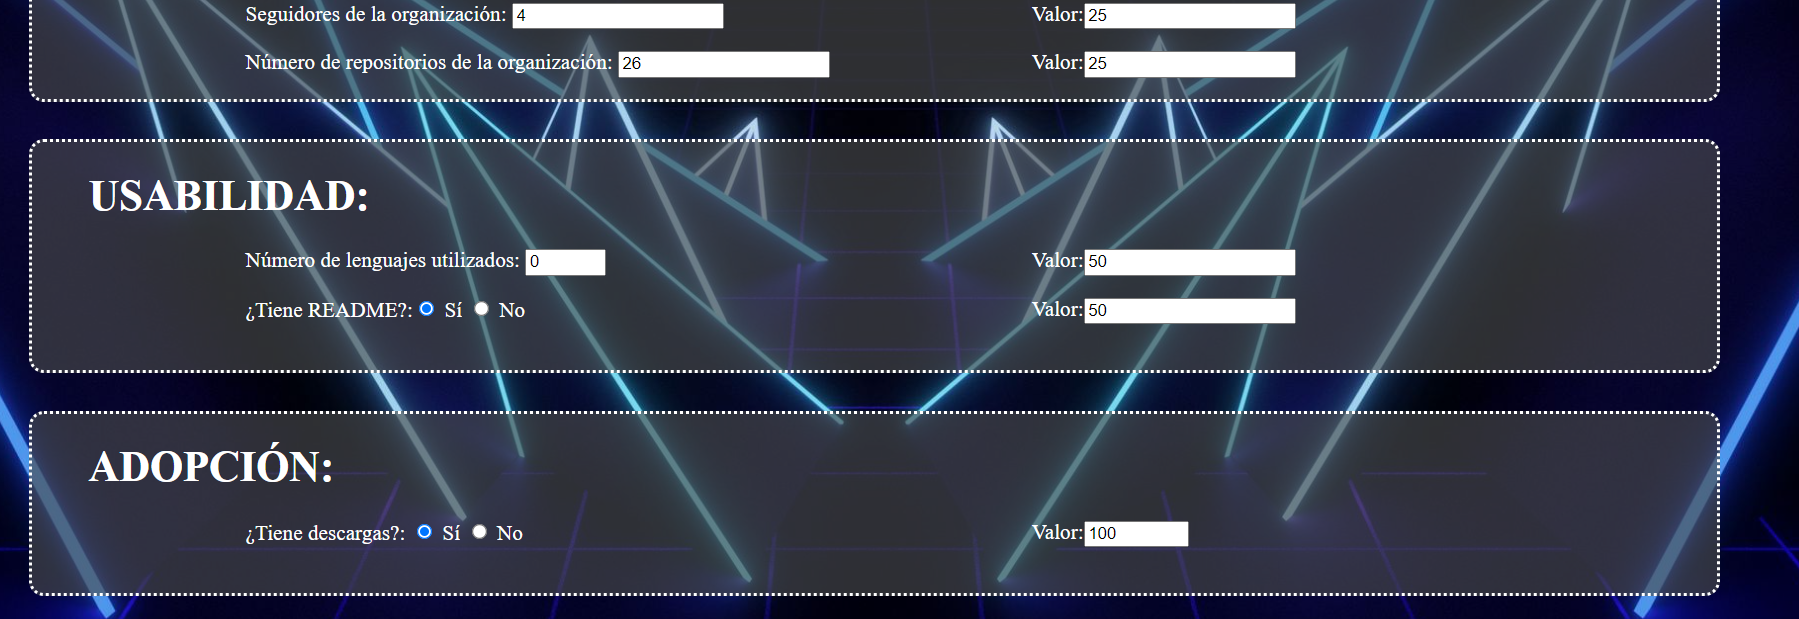
\includegraphics[ width=1.1\textwidth, keepaspectratio]{img/myteachingURJC_3.png}
    \caption{Datos del repositorio de ''Arquitectura de computadores''.}\label{fig:myteachingURJC_3}
\end{figure}

\subsection{Resultados de myTeachingURJC/Arq-computadores-01}

A continuación, se ven los resultados del análisis del repositorio. Véase de la figura~\ref{fig:myteachingURJC_4} a la figura~\ref{fig:myteachingURJC_6}. Obtenemos una calificación final de 3.13 sobre 5, lo que es una calificación coherente con este repositorio.

\begin{figure}
    \centering
    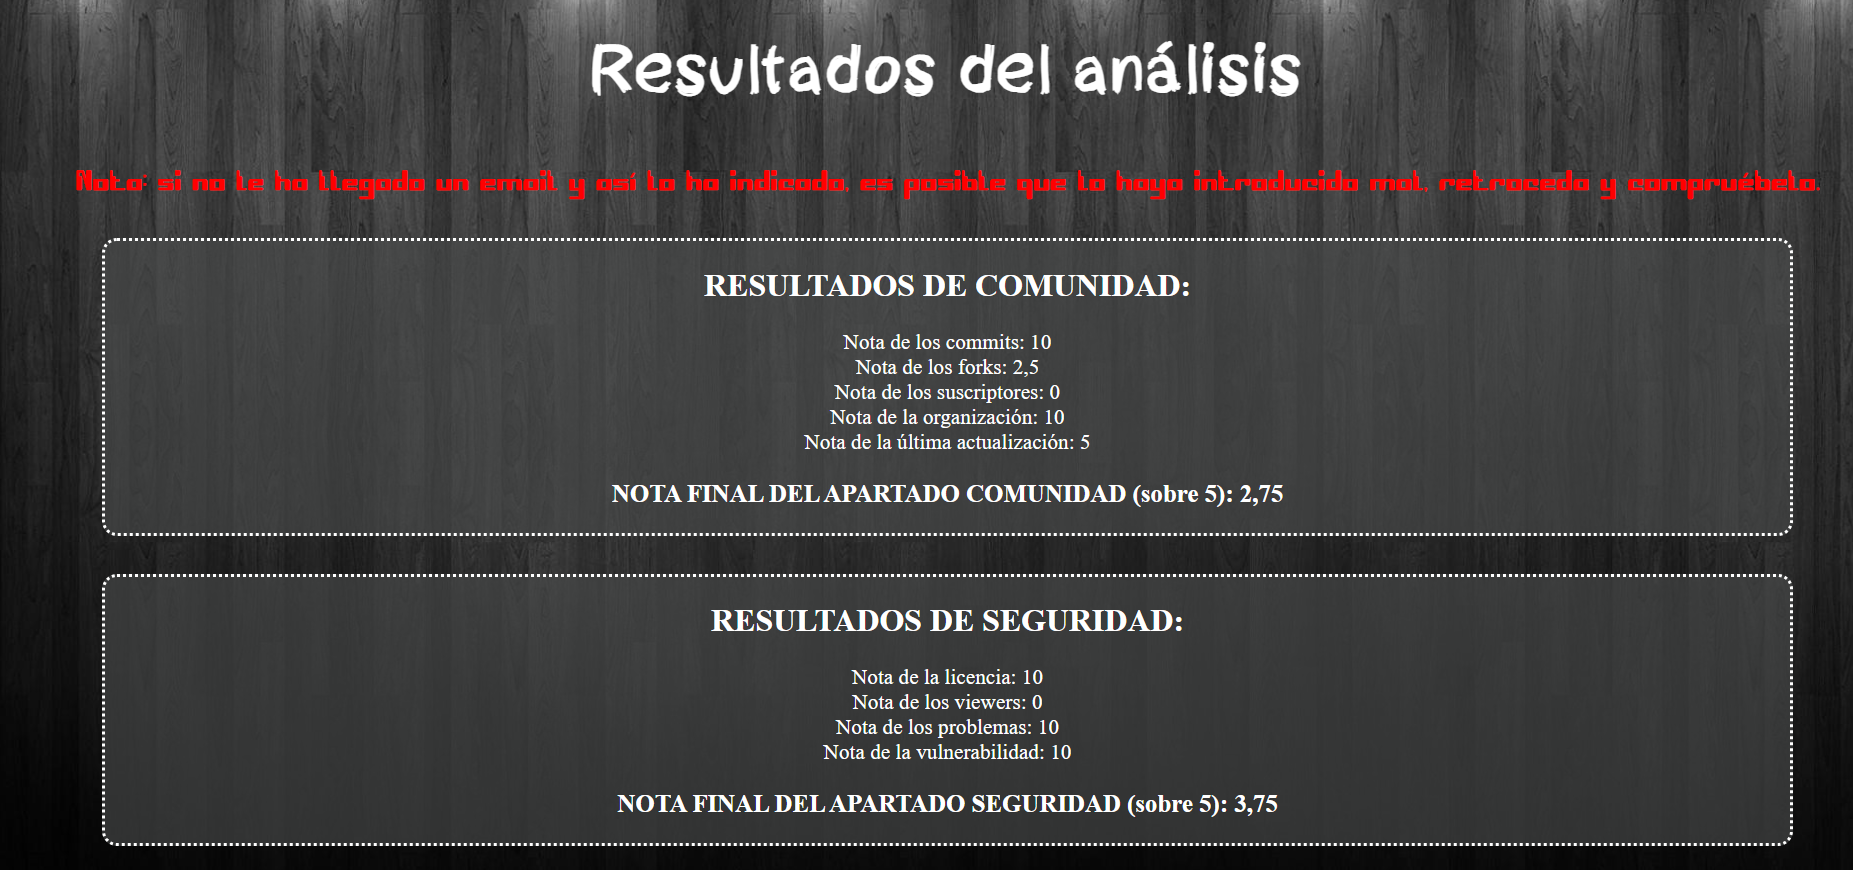
\includegraphics[ width=1.1\textwidth, keepaspectratio]{img/myteachingURJC_4.png}
    \caption{Resultados del repositorio de ''Arquitectura de computadores''.}\label{fig:myteachingURJC_4}
\end{figure}

\begin{figure}
    \centering
    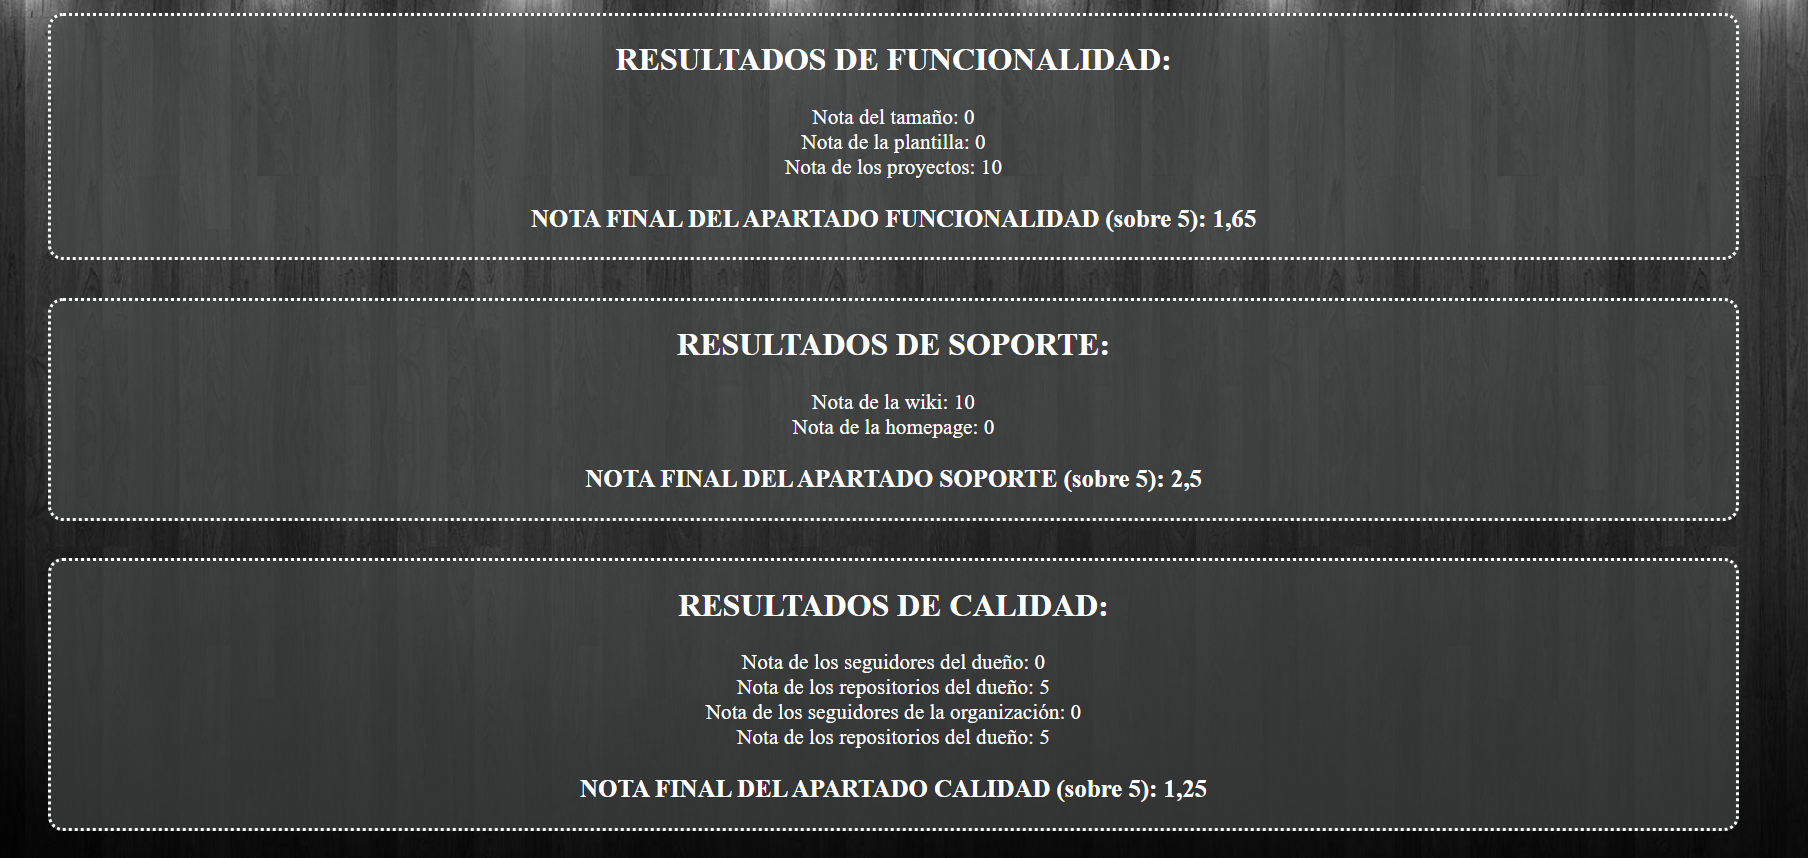
\includegraphics[ width=1.1\textwidth, keepaspectratio]{img/myteachingURJC_5.png}
    \caption{Resultados del repositorio de ''Arquitectura de computadores''.}\label{fig:myteachingURJC_5}
\end{figure}

\begin{figure}
    \centering
    
\includegraphics[ width=1.1\textwidth, keepaspectratio]{img/myteachingURJC_6.png}
    \caption{Resultados del repositorio de ''Arquitectura de computadores''.}\label{fig:myteachingURJC_6}
\end{figure}

\section{Prueba con moodle/moodle}

Ahora, vamos a probar con un repositorio teóricamente completo como es el de Moodle\footnote{\url{https://github.com/moodle/moodle}} que tenemos en la figura~\ref{fig:moodle}. Moodle\cite{website:Moodle}  es un sistema de gestión de aprendizaje, gratuito y de código abierto que utilizan muchos centros educativos. Por ejemplo, la URJC lo usa para la gestión de su Aula Virtual\footnote{\url{https://www.aulavirtual.urjc.es/moodle/login/index.php}} 

\begin{figure}
    \centering
    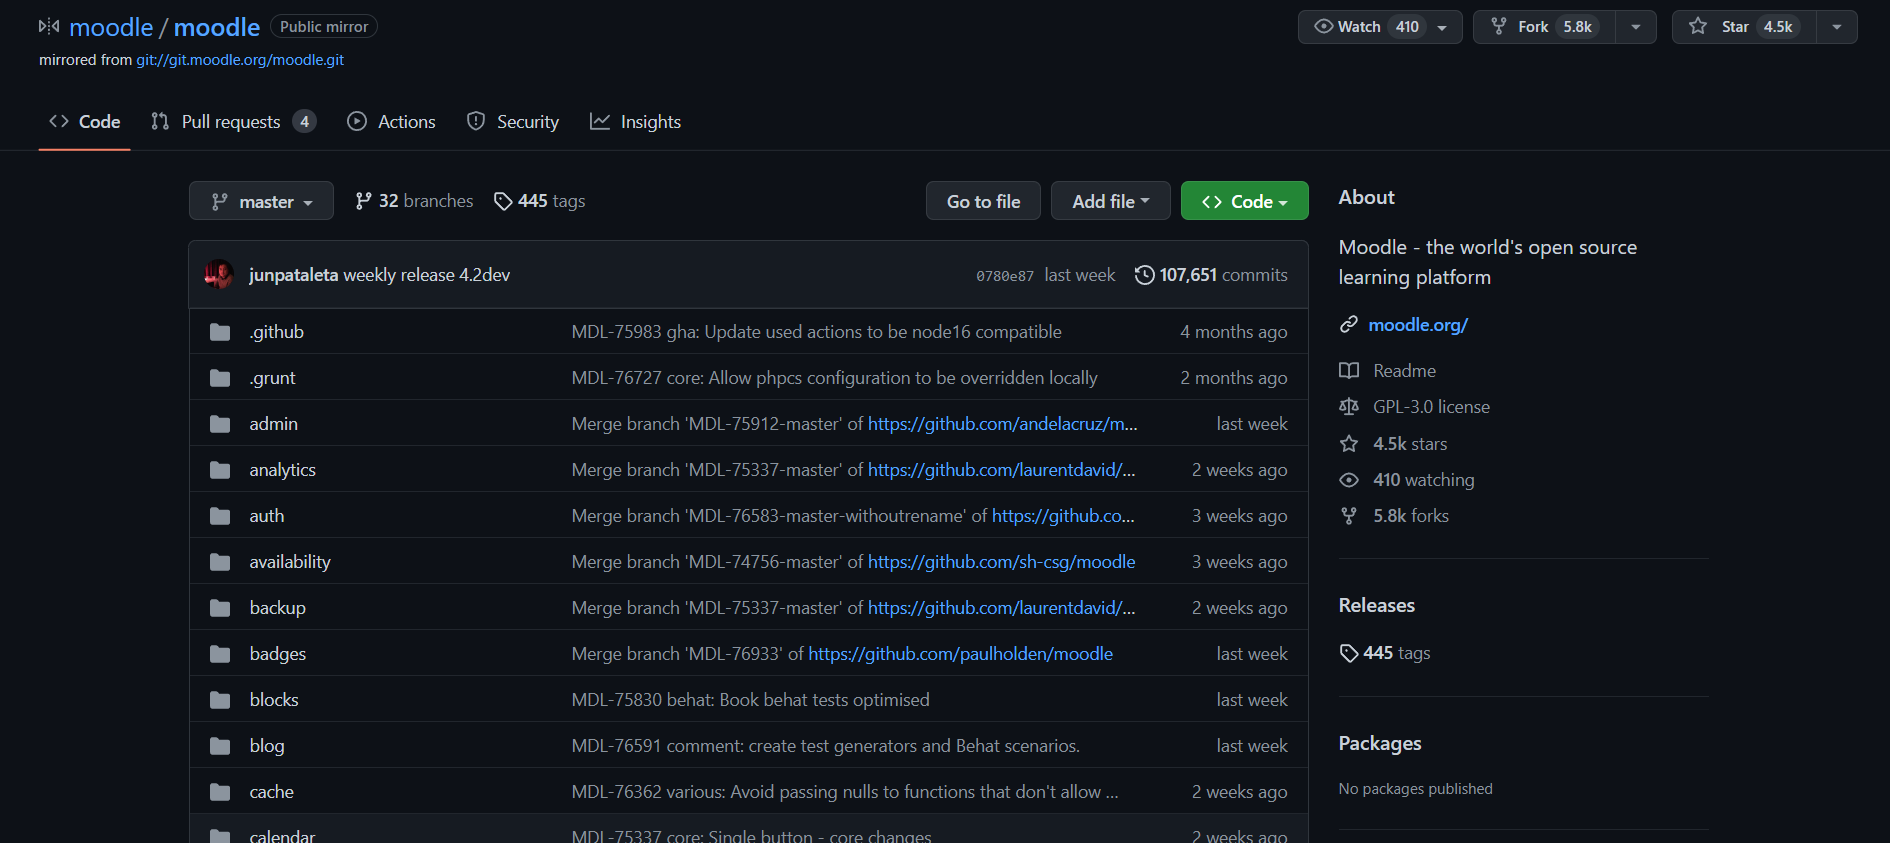
\includegraphics[ width=1.1\textwidth, keepaspectratio]{img/moodle.png}
    \caption{Vista inicial del repositorio de Moodle.}\label{fig:moodle}
\end{figure}

\subsection{Análisis de moodle/moodle}

Como siempre, en primer lugar obtenemos los datos del repositorio que mandaremos a través del formulario para su posterior calificación. Lo vemos de la figura~\ref{fig:moodle_1} a la figura~\ref{fig:moodle_3}.

\begin{figure}
    \centering
    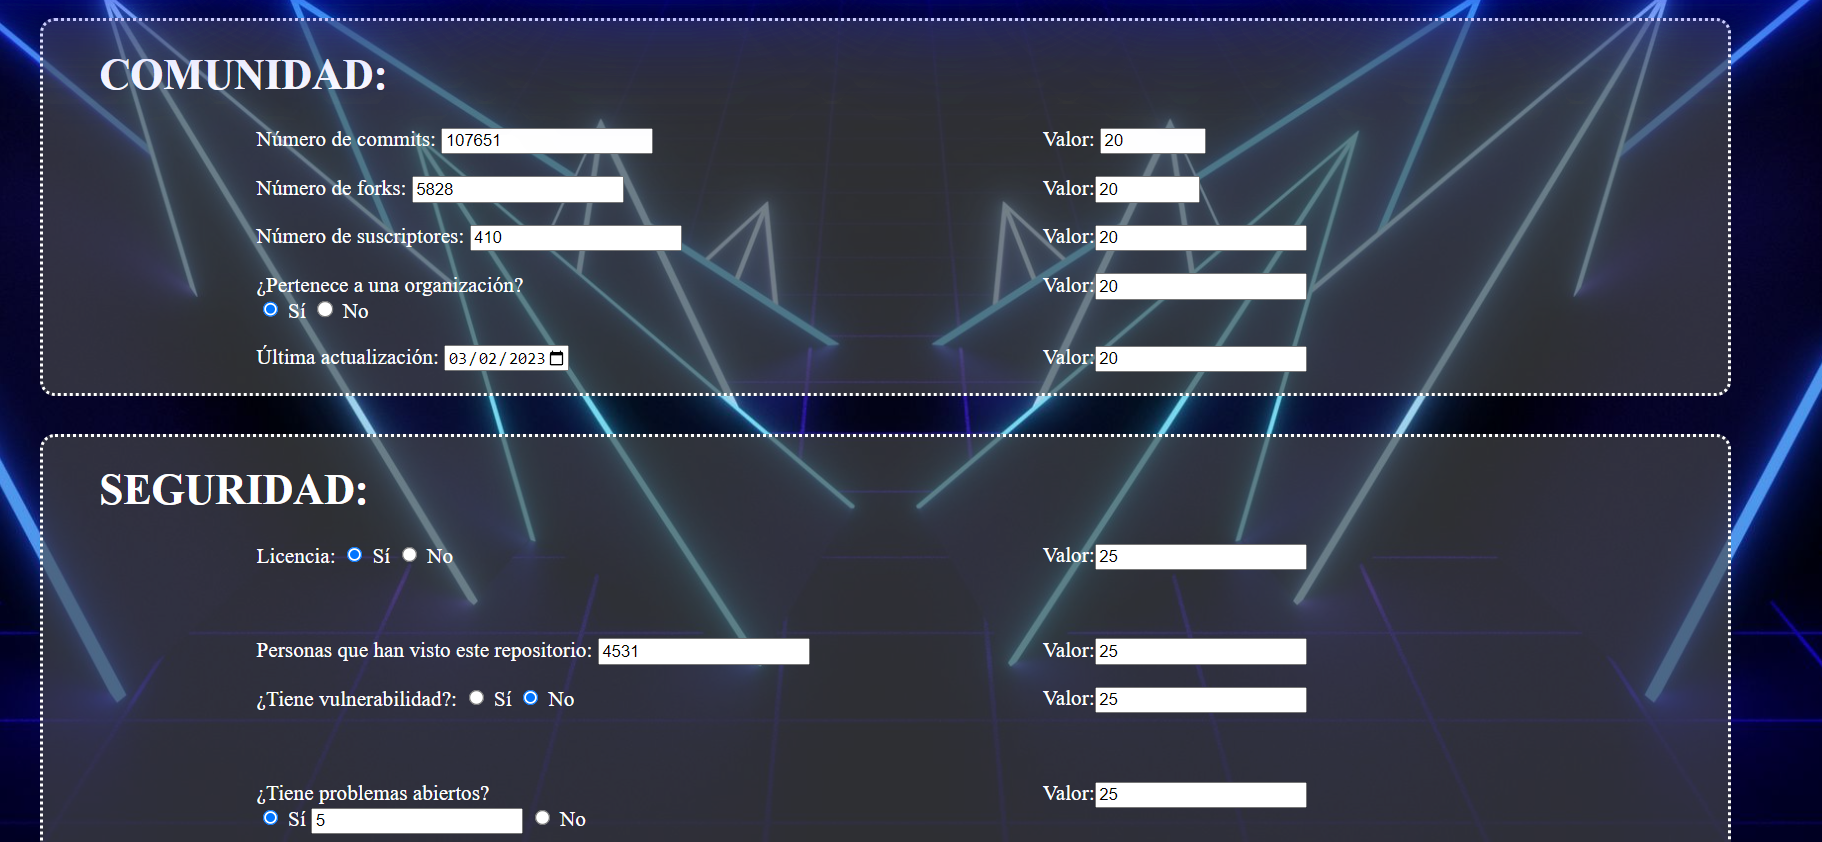
\includegraphics[ width=1.1\textwidth, keepaspectratio]{img/moodle_1.png}
    \caption{Datos del repositorio de Moodle.}\label{fig:moodle_1}
\end{figure}

\begin{figure}
    \centering
    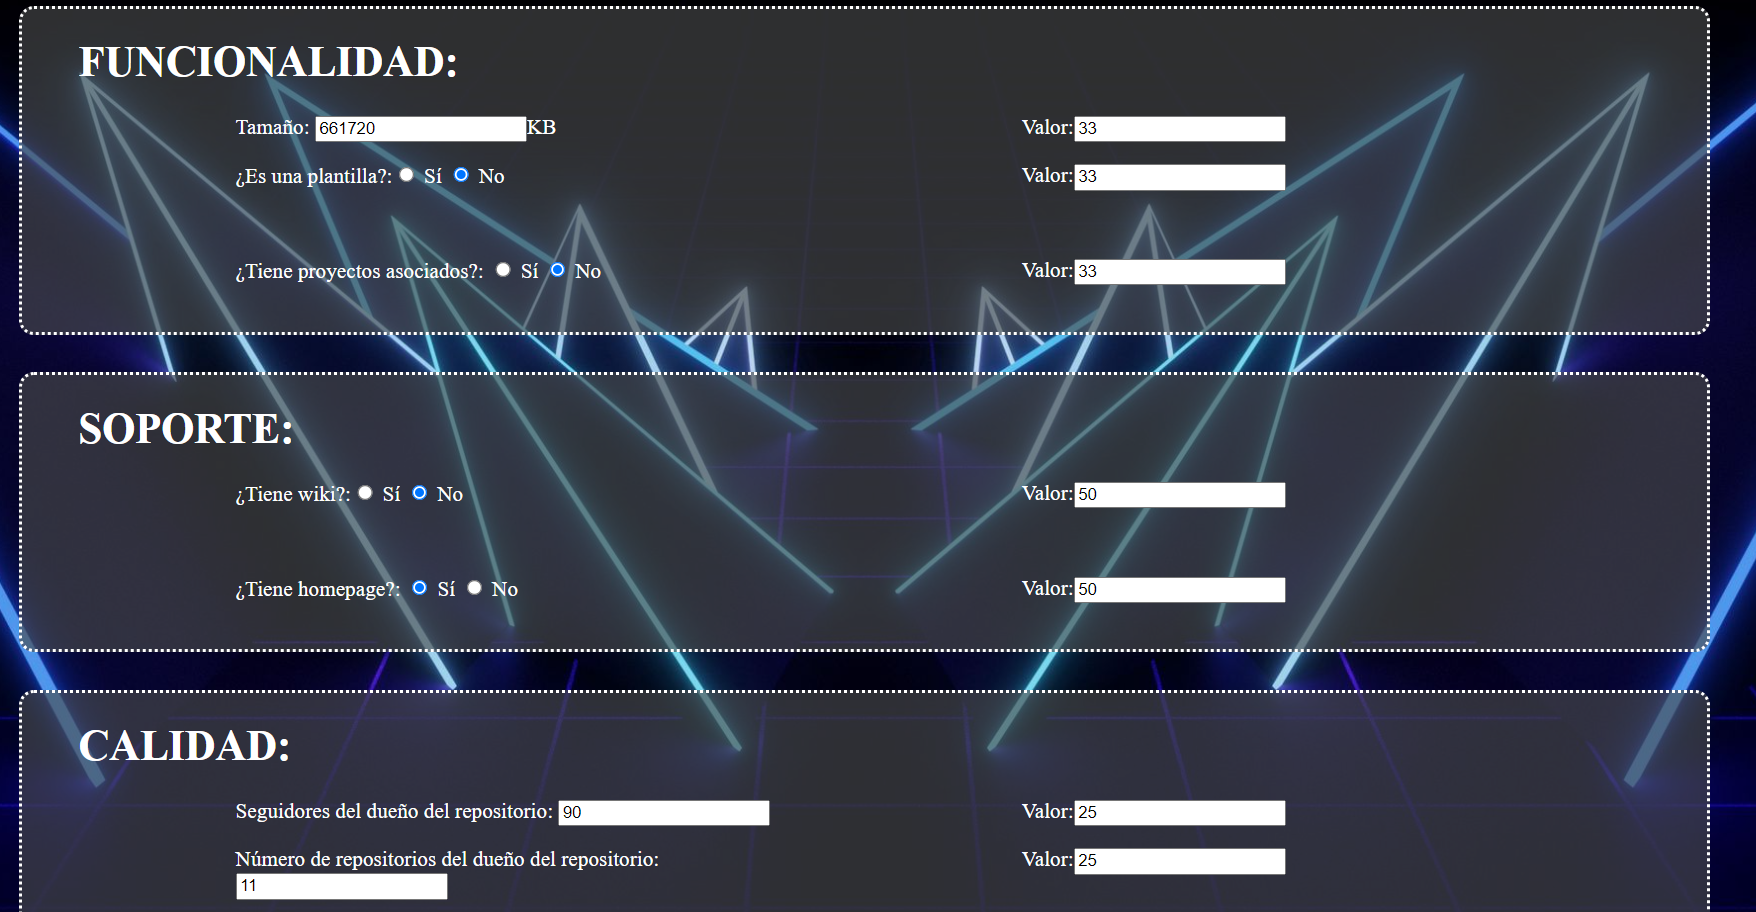
\includegraphics[ width=1.1\textwidth, keepaspectratio]{img/moodle_2.png}
    \caption{Datos del repositorio de Moodle.}\label{fig:moodle_2}
\end{figure}

\begin{figure}
    \centering
    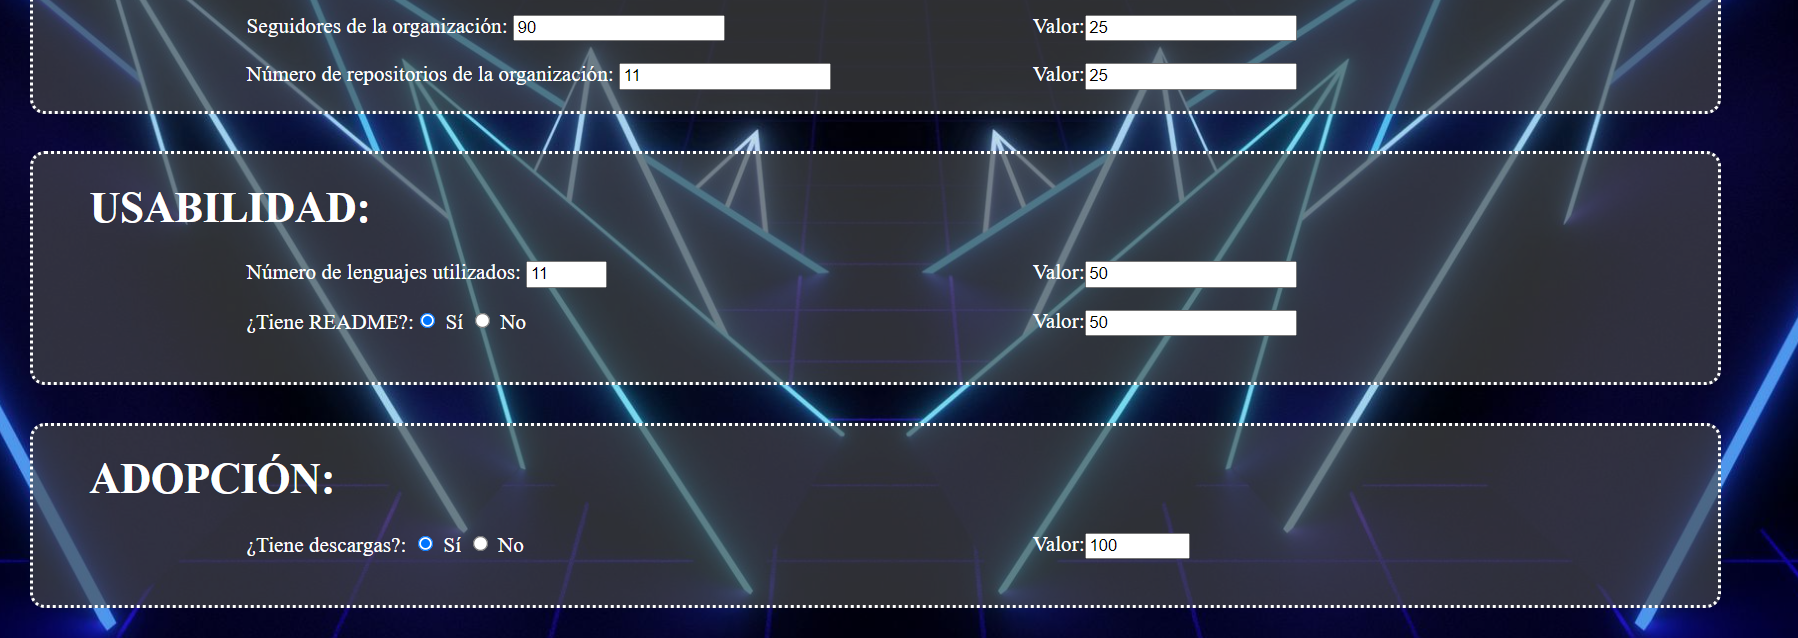
\includegraphics[ width=1.1\textwidth, keepaspectratio]{img/moodle_3.png}
    \caption{Datos del repositorio de Moodle.}\label{fig:moodle_3}
\end{figure}

\subsection{Resultados de moodle/moodle}

Finalmente, vemos los resultados del análisis del repositorio de Moodle. Véase de la figura~\ref{fig:moodle_4} a la figura~\ref{fig:moodle_6}. Obtenemos una calificación final de 3.09 sobre 5, lo que nos vuelve a indicar que es un buen repositorio, es decir, es de fiar.

\begin{figure}
    \centering
    \includegraphics[ width=1.1\textwidth, keepaspectratio]{img/moodle_4.png}
    \caption{Resultados del repositorio de Moodle.}\label{fig:moodle_4}
\end{figure}

\begin{figure}
    \centering
    \includegraphics[ width=1.1\textwidth, keepaspectratio]{img/moodle_5.png}
    \caption{Resultados del repositorio de Moodle.}\label{fig:moodle_5}
\end{figure}

\begin{figure}
    \centering
    \includegraphics[ width=1.1\textwidth, keepaspectratio]{img/moodle_6.png}
    \caption{Resultados del repositorio de Moodle.}\label{fig:moodle_6}
\end{figure}

\section{Prueba con un repositorio vacío}
\label{sec:vacio}

Finalmente, probaremos la aplicación con un repositorio que no contenga nada, únicamente el README inicial, para demostrar que mantiene la coherencia a la hora de calificar. Adicionalmente, se modificarán los datos para probar cómo cambian los resultados. El repositorio elegido para esta prueba es ''ivanmiguelmolinero/repositorio\textunderscore vacio''\footnote{\url{https://github.com/ivanmiguelmolinero/repositorio_vacio}}. Lo podemos ver en la figura~\ref{fig:vacio}.

\begin{figure}
    \centering
    \includegraphics[ width=1.1\textwidth, keepaspectratio]{img/vacio.png}
    \caption{Vista inicial del repositorio vacío.}\label{fig:vacio}
\end{figure} 

\subsection{Análisis del repositorio vacío}

Volvemos a ver los datos recogidos del análisis de un repositorio, esta vez del repositorio ''ivanmiguelmolinero/repositorio\textunderscore vacio''. Los datos van de la figura~\ref{fig:vacio_1} a la figura~\ref{fig:vacio_3}.

\begin{figure}
    \centering
    \includegraphics[ width=1.1\textwidth, keepaspectratio]{img/vacio_1.png}
    \caption{Datos del repositorio vacío.}\label{fig:vacio_1}
\end{figure}

\begin{figure}
    \centering
    \includegraphics[ width=1.1\textwidth, keepaspectratio]{img/vacio_2.png}
    \caption{Datos del repositorio vacío.}\label{fig:vacio_2}
\end{figure}

\begin{figure}
    \centering
    \includegraphics[ width=1.1\textwidth, keepaspectratio]{img/vacio_3.png}
    \caption{Datos del repositorio vacío.}\label{fig:vacio_3}
\end{figure}

\subsection{Resultados del repositorio vacío}

Vemos que los resultados son bastante peores en comparación con los dos casos anteriores, obteniendo una calificación final de 2.17, luego es una calificación coherente. Vemos los resultados de la figura~\ref{fig:vacio_4} a la figura~\ref{fig:vacio_6}.

\subsection{Modificación de los datos del repositorio vacío}

Como se indica en el apartado~\ref{sec:vacio} vamos a pasar a modificar los datos y los valores que hemos obtenido al analizar el repositorio vacío. Esta funcionalidad ha sido añadida para que el usuario pueda dar más importancia a la análisis de según que apartados según le convenga para sus menesteres o por si quiere comprobar como cambiaría la calificación de su repositorio en caso de que cambiara cosas antes de realizar esas modificaciones.
Se han modificado los datos de los parámetros de comunidad y seguridad (el resto se han dejado igual) como vemos en la figura~\ref{fig:vacio_7}.

Vemos en la figura~\ref{fig:vacio_8}, pues, que los resultados de estos parámetros han mejorado y consecuentemente la nota final del repositorio como se puede observar en la figura~\ref{fig:vacio_9}.

\begin{figure}
    \centering
    \includegraphics[ width=1.1\textwidth, keepaspectratio]{img/vacio_4.png}
    \caption{Resultados del repositorio vacío.}\label{fig:vacio_4}
\end{figure}

\begin{figure}
    \centering
    \includegraphics[ width=1.1\textwidth, keepaspectratio]{img/vacio_5.png}
    \caption{Resultados del repositorio vacío.}\label{fig:vacio_5}
\end{figure}

\begin{figure}
    \centering
    \includegraphics[ width=1.1\textwidth, keepaspectratio]{img/vacio_6.png}
    \caption{Resultados del repositorio vacío.}\label{fig:vacio_6}
\end{figure}	

\begin{figure}
    \centering
    \includegraphics[ width=1.1\textwidth, keepaspectratio]{img/vacio_7.png}
    \caption{Datos modificados del repositorio vacío.}\label{fig:vacio_7}
\end{figure}	

\begin{figure}
    \centering
    \includegraphics[ width=1.1\textwidth, keepaspectratio]{img/vacio_8.png}
    \caption{Resultados modificados del repositorio vacío.}\label{fig:vacio_8}
\end{figure}	

\begin{figure}
    \centering
    \includegraphics[ width=1.1\textwidth, keepaspectratio]{img/vacio_9.png}
    \caption{Resultados finales modificados del repositorio vacío.}\label{fig:vacio_9}
\end{figure}	

%%%%%%%%%%%%%%%%%%%%%%%%%%%%%%%%%%%%%%%%%%%%%%%%%%%%%%%%%%%%%%%%%%%%%%%%%%%%%%%%
%%%%%%%%%%%%%%%%%%%%%%%%%%%%%%%%%%%%%%%%%%%%%%%%%%%%%%%%%%%%%%%%%%%%%%%%%%%%%%%%
% CONCLUSIONES %
%%%%%%%%%%%%%%%%%%%%%%%%%%%%%%%%%%%%%%%%%%%%%%%%%%%%%%%%%%%%%%%%%%%%%%%%%%%%%%%%

\cleardoublepage
\chapter{Conclusiones}
\label{chap:conclusiones}

Tras la realización de este proyecto se han conseguido varios de los objetivos planteados inicialmente. En este capítulo se explicarán cuáles se han conseguido y cómo se han paliado los objetivos que no.

\section{Consecución de objetivos}
\label{sec:consecucion-objetivos}

En primer lugar se explicarán los objetivos conseguidos y a continuación la solución a los objetivos que no se han podido conseguir.

\subsection{Objetivos conseguidos}

\begin{itemize}
	\item Se ha aprendido a manejar Django gracias a los tutoriales de DjangoGirls recomendados al principio del proyecto por mi tutor.
	\item Se ha entendido la utilidad y necesidad de usar tecnologías como OpenBRR para poder analizar qué códigos y/o repositorios son mejores que otros. Hay una cantidad ingente de proyectos y estas tecnologías son necesarias para distinguir cuáles son los más válidos. OpenBRR hace un análisis inteligente ya que se basa en los parámetros más esenciales.
	\item La librería PyGithub se ha entendido a la perfección a la hora de sacar los datos necesarios para un análisis de repositorio. Esta librería también es útil para gestionar Github pero ha quedado pendiente aprender esta utilidad ya que no era necesaria para el proyecto.
	\item El envío de formularios con Django funciona correctamente en la aplicación.
	\item A la hora de modificar los datos se encontró el problema de que la aplicación no recordaba los cambios pero se pudo solucionar con las funciones ''save\textunderscore input'' de ''datos.js''.
	\item En un principio no sabía qué ponderación dar a cada dato/parámetro pero con ayuda de mi tutor decidimos que lo mejor es que el usuario decidiera este asunto por lo que se le dio la opción de poder modificarlo quedando un reparto equitativo como opción por defecto. Así se consiguieron resultados coherentes.
	\item Se solucionó error causado cuandoel usuario introduce un repositorio que no existe dándole la posibilidad de volver a la página inicial.
	\item Investigando las diversas funcionalidades de Django di con una que permitía el envío de correos por lo que decidí implementarlo de forma extra en mi proyecto para dar la posibilidad al usuario de guardar los resultados en un sitio seguro.
\end{itemize}

\subsection{Solución de los objetivos no conseguidos}

\begin{itemize}
	\item No se ha conseguido solucionar el error de PyGithub que limita el número de peticiones que puede realizar el usuario por lo que se ha puesto una pantalla de error que informa al usuario del error y le permite volver a la página principal indicándole que debe esperar antes de volver a analizar un repositorio.
	\item A la hora de mostrar y ocultar las pestañas en la pantalla de datos no se ha conseguido que el usuario pueda mandar los datos con las pestañas ocultas ya que la aplicación detecta que los formularios que están ocultos están vacíos por lo que se ha optado por no permitir al usuario enviar los datos con alguna pestaña oculta. Cuando lo intenta, se le muestra la alerta que vemos en la figura~\ref{fig:alerta}.
\end{itemize}

\begin{figure}
    \centering
    \includegraphics[ width=1.1\textwidth, keepaspectratio]{img/alerta.png}
    \caption{Alerta mostrada cuando hay una pestaña oculta.}\label{fig:alerta}
\end{figure}	

\section{Aplicación de lo aprendido}
\label{sec:aplicacion}

Para la realización de este TFG he aplicado los conocimientos adquiridos en las diferentes asignaturas de programación que hay durante el grado así como un asignatura de primero a la hora de redactar la memoria.

\begin{enumerate}
  \item \textbf{Expresión Oral y Escrita y Búsqueda de Información:} Me ha ayudado a realizar una correcta redacción de la memoria y buscar información de forma eficaz.
  \item \textbf{Informática I:} Cuando estudie esta asignatura en 2016, me enseñaron Picky pero aún así pude aprender los fundamentos de la programación y las sintaxis básicas.
  \item \textbf{Protocolos para la Transmisión de Audio y Vídeo en Internet:} En esta asignatura aprendí a programar en Python, el lenguaje con el que está desarrollada esta aplicación en su mayoría.
  \item \textbf{Construcción de Servicios y Aplicaciones Audiovisuales en Internet:} Gracias a esta asignatura aprendí HTML, CSS y Javascript y me inicié en el desarrollo web del lado del cliente. Con estos lenguajes funcionan las diferentes ventanas de este proyecto.
  \item \textbf{Laboratorio de Tecnologías Audiovisuales en la Web:} En esta asignatura aprendí a desarrollar el lado del servidor en una página web lo que ha sido de mucha ayuda a la hora de entender fácilmente Django.
\end{enumerate}


\section{Lecciones aprendidas}
\label{sec:lecciones_aprendidas}

Con lo aprendido durante el grado no fue suficiente así que tuve que adquirir diversos conocimientos para poder realizar el TFG.

\begin{enumerate}
  \item Aprender a gestionar y aprovechar mejor el tiempo en un proyecto más largo que cualquier trabajo de clase.
  \item Entender y utilizar Django.
  \item Entender y utilizar PyGithub.
  \item Avanzar en mis conocimientos de Github y aprender que no se trata simplemente de un repositorio donde subir tus proyectos si no que también ayuda a gestionarlos, buscar errores, colaborar con otros desarrolladores, etc.
  \item Aprender a realizar un manual de usuario.
  \item Afianzar mis conocimientos sobre programación y programar de una manera más limpia.
  \item Aprender a utilizar \LaTeX  para la redacción de la memoria.
\end{enumerate}


\section{Trabajos futuros}
\label{sec:trabajos_futuros}

Como todo proyecto de software, este TFG no está terminado ni mucho menos. Siempre se puede mejorar su optimización o añadir nuevas mejoras y funcionalidades. A continuación se mencionan algunas:

\begin{itemize}
	\item Corregir el error que no permite enviar el formulario si las pestañas están ocultas.
	\item Solucionar el error que limita el número de peticiones de PyGithub.
	\item Añadir una funcionalidad que permita comparar varios repositorios a la vez y que devuelva cuál es el mejor según la necesidad del desarrollador.
	\item Añadir más datos a analizar en cada parámetro de OpenBRR.
\end{itemize}


%%%%%%%%%%%%%%%%%%%%%%%%%%%%%%%%%%%%%%%%%%%%%%%%%%%%%%%%%%%%%%%%%%%%%%%%%%%%%%%%
%%%%%%%%%%%%%%%%%%%%%%%%%%%%%%%%%%%%%%%%%%%%%%%%%%%%%%%%%%%%%%%%%%%%%%%%%%%%%%%%
% APÉNDICE(S) %
%%%%%%%%%%%%%%%%%%%%%%%%%%%%%%%%%%%%%%%%%%%%%%%%%%%%%%%%%%%%%%%%%%%%%%%%%%%%%%%%

\cleardoublepage
\appendix
\chapter{Manual de usuario}
\label{app:manual}

Esta aplicación permite analizar un repositorio de Github según los parámetros de OpenBRR.

\section{Instalación}

Para instalar y poder usar esta aplicación en tu ordenador personal debes dirigirte al repositorio ''ivanmiguelmolinero/TFG''\footnote{\url{https://github.com/ivanmiguelmolinero/TFG}} y clonarlo en un directorio local. A continuación deberás instalar Django en tu entorno. Para ello abre una ventana de comandos y ejecuta el siguiente comando:

\begin{verbatim}
pip install django
\end{verbatim}

Se empezará a instalar y, una vez te indique que la instalación ha sido realizada con éxito, estará todo listo para comenzar a usar la aplicación.

\subsection{Configuración del correo.}

Para configurar la funcionalidad del envío del correo tendremos que dirigirnos a la carpeta ''mysite'' y:

\begin{enumerate}
	\item En el fichero settings.py cambiar el valor de ''EMAIL\textunderscore HOST\textunderscore USER'' por tu propia dirección de correo.
	\item Crear un fichero ''credentials.env'' donde introduciremos lo siguiente:
	\begin{verbatim}
	EMAIL_USER = ejemplo@gmail.com
	EMAIL_PASSWORD = contraseña
	\end{verbatim}
	\item El valor del campo contraseña se obtiene en \url{https://myaccount.google.com/security} en el apartado ''Iniciar sesión en Google'' $">"$ ''Contraseñas de aplicaciones''.
\end{enumerate}

\section{Iniciar la aplicación.}

Para iniciar la aplicación debes abrir una ventana de comandos en la carpeta ''Django\textunderscore BRR'' y ejecutar:

\begin{verbatim}
python manage.py runserver
\end{verbatim}

\section{Uso de la aplicación.}

Finalmente para utilizar esta aplicación, abrimos un navegador y nos dirigimos a la dirección ''http://127.0.0.1:8000/'' y se nos abrirá la ventana principal (figura~\ref{fig:pricipal_pygithub}).

Una vez ahí, podremos introducir el repositorio que queramos analizar siguiendo la estructura ''usuario/nombre\textunderscore del\textunderscore repositorio'' por ejemplo ''ivanmiguelmolinero/TFG'' donde ivanmiguelmolinero es el usuario del dueño del repositorio y TFG el nombre del repositorio. Pulsamos en ''ANALIZAR'' y nos llevará a la siguiente ventana.

Ya en la ventana de datos (de la figura~\ref{fig:moodle_1} a la figura~\ref{fig:moodle_3}) nos aparecerán los 7 parámetros analizados ocultos en sus correspondientes pestañas. Para poder verlo debemos pulsar en sus correspondientes botones. Podemos cambiar los datos analizados e incluso la ponderación que aporta cada uno. Al final de esta página, de manera opcional, podremos introducir una dirección de correo a la que nos llegaría un mensaje con los resultados del análisis. Pulsamos en ''ENVIAR DATOS'' y nos llevará a la última ventana.

Finalmente, en la ventana de resultados (de la figura~\ref{fig:moodle_4} a la figura~\ref{fig:moodle_6}), vemos la calificación de cada apartado y la calificación final del repositorio.

%%%%%%%%%%%%%%%%%%%%%%%%%%%%%%%%%%%%%%%%%%%%%%%%%%%%%%%%%%%%%%%%%%%%%%%%%%%%%%%%
%%%%%%%%%%%%%%%%%%%%%%%%%%%%%%%%%%%%%%%%%%%%%%%%%%%%%%%%%%%%%%%%%%%%%%%%%%%%%%%%
% BIBLIOGRAFIA %
%%%%%%%%%%%%%%%%%%%%%%%%%%%%%%%%%%%%%%%%%%%%%%%%%%%%%%%%%%%%%%%%%%%%%%%%%%%%%%%%

\cleardoublepage

% Las siguientes dos instrucciones es todo lo que necesitas
% para incluir las citas en la memoria
\bibliographystyle{abbrv}
\bibliography{memoria}  % memoria.bib es el nombre del fichero que contiene
% las referencias bibliográficas. Abre ese fichero y mira el formato que tiene,
% que se conoce como BibTeX. Hay muchos sitios que exportan referencias en
% formato BibTeX. Prueba a buscar en http://scholar.google.com por referencias
% y verás que lo puedes hacer de manera sencilla.
% Más información: 
% http://texblog.org/2014/04/22/using-google-scholar-to-download-bibtex-citations/

\end{document}
